\section{The missing link is construction, not another
certificate}\label{finding}

The strongest new finding is specific. A critic can now produce a
failure witness that becomes an executable constraint in the same
mission that produced the faulty schedule. The compiler does not merely
name a better method: it creates a numerical operation, applies it, and
returns a different dispatch artifact. A separate checker then evaluates
the artifact against the original obligations. This closes a real
implementation gap in the inspected developer source.

The strongest comparator is equally important. A conventional linear
program, given the same finite task and complete constraint set, already
produces an accepted answer on every task in the new panel. The
corrective procedure does not open a new feasible activity relative to
that comparator. It reconstructs constraints that the comparator can
incorporate directly, and its measured overhead is higher. A successful
repair is therefore not automatically a useful invention advantage.

The economic evidence narrows the conclusion further. In a separately
recovered structural-transfer campaign, all five technical arms produce
the same accepted classification counts. The current instrument ledger
is loss-making after its recorded late expenses, and its funded control
performs no worse on the successor comparison. None of the newly
screened real-world prospects has an admitted cohort whose baseline loss
and treatment profit are both supported by complete evidence. These are
three distinct boundaries---technical attribution, economic
identification, and source completeness---not one generic lack of
confidence.

This edition does not substitute the reserve-scheduling fixture for the
intended business transformation. It uses the fixture to close the
constructive feedback defect, preserves the conventional winner, audits
the existing commercial evidence, and identifies precisely what a
substantive next campaign must establish. The implementation and checks
are part of the contribution; the manuscript records them.

\subsection{Research questions and decision
standard}\label{research-questions-and-decision-standard}

We distinguish three questions that are often collapsed into the phrase
``the flywheel works.'' First, can verified criticism cause an actual
executable correction? Second, can that correction, structural transfer,
or accumulated experience outperform the strongest competent complete
workflow under comparable information and resources? Third, does the
improvement turn the \emph{same admitted activity and cohort} from
negative to positive complete-cost profit, leaving settled surplus that
finances a useful additional construction?

Only the first question receives a positive bounded answer here. The
second receives a negative result on the new finite panel and remains
unestablished more broadly. The third is not identified for a real
cohort and is not supported by the recovered simulated instrument
accounts. This distinction avoids dismissing useful engineering while
preventing a component result from being promoted into a business or
intelligence claim.

For clarity, ``invention'' in the narrow implementation result means a
newly constructed task-specific executable artifact relative to the
inspected predecessor. It does not mean a new theorem, a previously
unknown optimization algorithm, an autonomously invented physical
mechanism, or worldwide scientific priority. The writer supplied the
compiler architecture and allowed operation language; the program
generated numerical constraints and schedules within that language.

\section{Continuity: what the existing series already
established}\label{continuity}

The series is an input to this work, not a collection of titles to
repeat. We inspected canonical source identities, the available full
manuscripts, bibliographies, code, and retained evidence at their actual
scope. Two complete local TeX sources match their canonical Git blobs
exactly. A third full TeX manuscript was recovered and likewise matched.
The retained \emph{Out-Evolve} PDF is complete, but its local TeX root
contains unresolved section inputs; we do not claim that its source
package can be rebuilt from the recovered root alone. Appendix A records
these limits.

\subsection{Four inherited
contributions}\label{four-inherited-contributions}

\emph{Transformational Intelligence: Learning to Change the Game}
separates authorized purpose from inherited formulation and evaluation.
Its exact two-world example has a passive-information ceiling of one
half and an intervention policy with accuracy \(8191/8192\) under at
most twelve queries. An unrestricted optimal planner matches the result.
The reusable lesson is a purpose-preserving formulation change with an
explicit information bridge, not a claim that an LLM discovered a new
causal algorithm. Its local exact-model code and bibliography were
inspected (\citeproc{ref-ti}{Boucher 2026d}).

\emph{Invent the Economy} makes technical and contractual arrangements
jointly editable. A supplied four-buyer example supports a shared
construction under assumed values and success probability, while cash
timing can still prevent entry. Its 2,240-case finite grid and
independently implemented event checker do not establish real buyer
commitments. We retain the separation of technical correctness,
participant acceptance, operating contribution, financing, and realized
exchange; we do not reuse its hypothetical prices as current demand
(\citeproc{ref-economy}{Boucher 2026b}).

\emph{Out-Evolve} asks what must be built to make subsequent discovery
possible. Its conditional response-family calculation contrasts
\(2^{20}=1,048,576\) arbitrary binary-configuration readings with
\(1+20+190=211\) readings when a qualified degree-two structure
genuinely holds. The structure must be earned, not assumed from
modular-looking components. Its compatible-extension argument and
retained operator work motivate construction prerequisites and
mission-relative revalidation. They are not a measured industrial
speedup or a physical platform constructed in this campaign
(\citeproc{ref-evolve}{Boucher 2026c}).

The canonical \emph{Autonomous Enterprises: Build the Means of Building}
makes inheritance operational in a bounded arithmetic foundry. It
reports that an inherited convolution program reduces a specified
inverse construction and qualification from 78,016 to 30,912 declared
work units. Joint construction costs 808,420 rather than 1,226,276 units
under the stated isolated-build comparison; unrestricted joint planning
matches it. Those are counted operations under supplied classical
templates, not currency or proof that an autonomous invention policy is
superior. We recovered its full canonical TeX, including the
bibliography and limitations, but not its matching complete foundry
companion. These figures remain attributed historical results, not a
fresh writer reproduction (\citeproc{ref-enterprise}{Boucher 2026a}).

\begin{longtable}[]{@{}
  >{\raggedright\arraybackslash}p{(\columnwidth - 6\tabcolsep) * \real{0.2500}}
  >{\raggedright\arraybackslash}p{(\columnwidth - 6\tabcolsep) * \real{0.2500}}
  >{\raggedright\arraybackslash}p{(\columnwidth - 6\tabcolsep) * \real{0.2500}}
  >{\raggedright\arraybackslash}p{(\columnwidth - 6\tabcolsep) * \real{0.2500}}@{}}
\caption{Continuity matrix. Earlier numerical claims retain their
original evidence class; this edition does not count them as new
experiments.}\tabularnewline
\toprule\noalign{}
\begin{minipage}[b]{\linewidth}\raggedright
Earlier claim / artifact
\end{minipage} & \begin{minipage}[b]{\linewidth}\raggedright
Demonstrated scope
\end{minipage} & \begin{minipage}[b]{\linewidth}\raggedright
Unresolved limitation
\end{minipage} & \begin{minipage}[b]{\linewidth}\raggedright
Reuse and new test
\end{minipage} \\
\midrule\noalign{}
\endfirsthead
\toprule\noalign{}
\begin{minipage}[b]{\linewidth}\raggedright
Earlier claim / artifact
\end{minipage} & \begin{minipage}[b]{\linewidth}\raggedright
Demonstrated scope
\end{minipage} & \begin{minipage}[b]{\linewidth}\raggedright
Unresolved limitation
\end{minipage} & \begin{minipage}[b]{\linewidth}\raggedright
Reuse and new test
\end{minipage} \\
\midrule\noalign{}
\endhead
\bottomrule\noalign{}
\endlastfoot
Purpose-preserving formulation; \emph{Transformational Intelligence} &
Exact passive/interventional finite model; unrestricted planner matches
& No autonomous discovery or physical experiment & Keep intent and final
acceptance fixed while compiling corrections \\
Contractual + technical complementarity; \emph{Invent the Economy} &
Supplied buyer-value grid and cash-timing checks & Demand and
participation remain modeled & Audit escrow, reserves and complete-cost
crossing separately \\
Construct means of discovery; \emph{Out-Evolve} & Conditional low-order
response family and retained operation & Physical family membership and
complete editable source not recovered & Treat prerequisites and
revalidation as obligations, not inherited truth \\
Capability-producing inheritance; \emph{Autonomous Enterprises} &
Measured arithmetic construction/qualification; joint planner matches &
Canonical companion not rerun; no external business validation & Compare
constructed successor against competent funded control \\
\end{longtable}

\subsection{What this paper adds---and does not
add}\label{what-this-paper-addsand-does-not-add}

The present addition is the executable path from a scalar failure
witness to a typed constraint and a regenerated artifact. It reuses the
developer's task model, baseline solver, workbench, mission compiler,
final checker, and evidence-pack format. It also adds read-only
reconstruction of the new constraints using an algebraically different
coefficient calculation, plus reconciliation of the latest available
commercial ledger rather than an obsolete positive checkpoint.

It does not claim to re-establish every preceding theorem or to
reproduce every earlier large experiment. It does not add a learned
physical observation channel, a qualified real business cohort, or a
demonstrated better invention policy. Recovered source is not
automatically installed authority. The newly located original SUCCESSOR
Omega Strategy Laboratory v0.1.0 is a separate bounded research
prototype: its 51 tests pass in this environment, but its 193,536
historical policy/control executions were not all rerun. Its validated
expression grammar, evolutionary search, frozen candidates, and
rejection of unsupported promotions are useful precedents, not evidence
that AGI ALPHA already possesses general strategy invention
(\citeproc{ref-omega}{SUCCESSOR Omega Strategy Laboratory 2026}).

\section{Source truth, architecture, and experimental
custody}\label{custody}

\subsection{Four evidence lineages, kept
separate}\label{four-evidence-lineages-kept-separate}

The supplied and recovered material contains related but nonidentical
studies. Combining their counts would manufacture a larger experiment
than actually occurred.

\begin{longtable}[]{@{}
  >{\raggedright\arraybackslash}p{(\columnwidth - 4\tabcolsep) * \real{0.3333}}
  >{\raggedright\arraybackslash}p{(\columnwidth - 4\tabcolsep) * \real{0.3333}}
  >{\raggedright\arraybackslash}p{(\columnwidth - 4\tabcolsep) * \real{0.3333}}@{}}
\caption{Separate evidence lineages. Records, tasks, constraints, and
orders are different denominators.}\tabularnewline
\toprule\noalign{}
\begin{minipage}[b]{\linewidth}\raggedright
Lineage
\end{minipage} & \begin{minipage}[b]{\linewidth}\raggedright
Available evidence
\end{minipage} & \begin{minipage}[b]{\linewidth}\raggedright
What this edition verified
\end{minipage} \\
\midrule\noalign{}
\endfirsthead
\toprule\noalign{}
\begin{minipage}[b]{\linewidth}\raggedright
Lineage
\end{minipage} & \begin{minipage}[b]{\linewidth}\raggedright
Available evidence
\end{minipage} & \begin{minipage}[b]{\linewidth}\raggedright
What this edition verified
\end{minipage} \\
\midrule\noalign{}
\endhead
\bottomrule\noalign{}
\endlastfoot
Original A/S/C and learning study & Source + aggregate tables; full
2,184-record archive missing & 71 tests; mechanism inspection; aggregate
arithmetic only \\
Structural transfer version 3 & Raw tasks, artifacts, source freezes,
SIM databases & 128 certificates; three latest financial snapshots \\
Invention-automation first cycle & Opportunity registry + three-case
fixture & Five tests; no real admitted cohort \\
Writer correction versions 1 and 2 & 72 tasks, 288 records, all traces
and native packs & 288 native replays; 1,220 generated rows; 72 optimum
rechecks \\
\end{longtable}

The first lineage is the original compounding-discovery source and
aggregate tables. The supplied answer reports a 2,184-case fixed panel
and interrupted predecessor runs, but the large complete raw archive was
not mounted and was not recovered from the visible Library search. We
reran its 71 tests and inspected its mechanisms. We can verify
arithmetic consistency in its CSV summaries, not reconstruct its
original pairing, bootstrap intervals, exposure history, or every native
pack. Its numerical findings are therefore explicitly \emph{reported
historical results} throughout this edition (\citeproc{ref-dev}{AGI
ALPHA development record 2026a}).

The second lineage is a recovered structural-transfer package with
actual per-task artifacts, source freezes, a saved checker, a
protected-exchange simulation, and SQLite histories. We replayed 128
certificates and independently recomputed the latest financial snapshots
from the databases. This package supports a stronger artifact-level
audit, but its numerical market assumptions remain simulation
assumptions (\citeproc{ref-transfer}{AGI ALPHA development record
2026c}).

The third lineage is the invention-automation first-cycle registry. It
has executable software and a small economic fixture, but all real
opportunities are UNKNOWN. Its useful role is to preserve screening
choices and expose what has not yet been admitted
(\citeproc{ref-firstcycle}{AGI ALPHA development record 2026b}). The
fourth lineage is the new writer extension and its two explicitly
exploratory pilots. Every new task, result, witness, constraint,
protocol, native pack, and read-only audit is included.

\subsection{Repository identities and authority
boundaries}\label{repository-identities-and-authority-boundaries}

The Alpha source base is commit
\path{12770c22b4a9f90f2013bbfb64242f912ba5071e}. The delivered
development workspace is a sparse reconstruction with exact required
upstream dependencies, not a full clone or a clean release checkout. The
original archive's 68 available source entries still match byte-for-byte
after the additive work. The new code is isolated under
\texttt{studies/agi-alpha-compounding-discovery-v1/writer\_extension/};
the paper occupies a new subdirectory of that same study.

Current repository metadata was read through the connected GitHub
interface. The inspected Fleet, Jobs, and Manager heads are recorded in
Appendix A. Fleet's instructions preserve inactive restores,
source-pinned qualification, STOP records, and explicit spending
authority. The Jobs and Manager discovery receivers declare local
inspection, unsupported submission, unprovisioned external execution,
and no authority. Their currency routes are alternatives:
\texttt{jobs-agialpha} / \texttt{AGIALPHA18} and \texttt{manager-usdc} /
\texttt{USDC6}, not two charges for one job. Root \texttt{AGENTS.md}
retrieval returned 404 for Jobs and Manager; relevant source and README
boundaries were inspected instead. We did not run their complete native
acceptance suites or claim that these routes were commissioned.

The new experiment uses the actual Alpha \texttt{createWorkbench}
interface, not a replacement simulator with a similar name. It emits
seven-node compiled job graphs, mission/release/integrity digests, an
inspectable \texttt{dispatch.json}, and the original local-execution
restrictions. Pack inspection verifies identities and bindings; it
labels imported evidence \texttt{UNAUTHENTICATED\_HISTORICAL\_IMPORT}.
Final records retain \textbf{admission HOLD}, \textbf{settlement
NOT\_CONNECTED}, and no active authority. An intact digest proves byte
identity, not physical validity, customer acceptance, or external
reviewer independence.

\subsection{Procedural separation, not institutional
independence}\label{procedural-separation-not-institutional-independence}

The builder does not receive the evaluation optimum. The final
JavaScript checker is unchanged and calculates trajectories directly. A
separately assembled Python matrix formulation provides the optimum
reference. The witness adjudicator does not import the builder or
solver. A later read-only audit recomputes generated coefficients using
closed products of retention factors rather than the builder's
forward-vector recurrence.

These separations help expose implementation errors, but all roles
operated in one AI-assisted session and share the same machine, task
specification, and numerical libraries. Both linear-program formulations
use HiGHS. No independent institution certified the result. Furthermore,
hashes do not create access control: the builder and checker files are
locally administered. The protocol records that outputs were not used
for within-panel tuning, not that a separate security domain
cryptographically concealed every case from the authoring process.

\section{Opportunity admission before economic
transformation}\label{opportunities}

The central business question is whether an instrument can make an
important previously unprofitable activity profitable. That question
needs an identified operator, activity, input cohort, ownership
boundary, service obligation, location, horizon, and best existing
complete route. The recovered opportunity registry does not yet supply
that complete object for any of its three prospects. A promising
bottleneck is not a demonstrated negative-profit cohort.

\subsection{Battery second life}\label{battery-second-life}

The candidate beneficiary is a repurposer deciding how to qualify and
route retired packs into a specified storage service. The material
questions include acquisition price, remaining life, diagnosis,
handling, safety qualification, assembly, warranty, and terminal
disposal. Cobb and colleagues model maximum acquisition prices using a
process-based repurposing model and life-adjusted comparison with new
storage; the institutional abstract supports chemistry- and
application-dependent economics, not a universal loss statement or a
current supplier quote (\citeproc{ref-cobb}{Cobb et al. 2026}). The PNNL
charging-station study is another existing techno-economic route, not an
unserved blank slate (\citeproc{ref-charging}{Gautam et al. 2025}).

Virtual reference electrodes are already published prior art. The
inspected abstract describes estimating an internal electrode state from
ordinary cell signals after training on specially measured cells. We
neither constructed that instrument nor validated its use on retired
heterogeneous packs (\citeproc{ref-virtual}{Yu et al. 2026}). An
admissible comparison must include competent diagnosis, whole-pack reuse
where feasible, recycling, and life-adjusted new storage. Without actual
asset condition, ownership, acquisition, warranty, and buyer
obligations, neither the baseline loss nor the treatment's break-even
bound can be identified. Status: \textbf{UNKNOWN}, not rejected and not
promoted.

\subsection{Difficult textile
recovery}\label{difficult-textile-recovery}

The proposed operator is a sorter or recycler facing a specified
difficult feedstock and an accepted output-purity requirement. Existing
NIR methods and NIST's NIR-SORT reference database are incumbent
resources, not new inventions by the campaign
(\citeproc{ref-nist}{National Institute of Standards and Technology
2025}). IOM's research description identifies difficulties with
carbon-black textiles and small elastane fractions while describing an
ongoing instrument-development program; it does not validate this
campaign's sensor, yield, throughput, or economics
(\citeproc{ref-iom}{IOM Leipzig 2025}).

A potentially consequential construction would change what is observable
or separable while preserving downstream quality. The aluminum-sorting
precedent is instructive: PNNL describes chemically changing an alloy's
observable appearance and using optical sorting. This is existing work,
not a transferable guarantee for textiles and not our invention
(\citeproc{ref-alloy}{Efe et al. 2025}). No new reagent, instrument,
textile measurement, batch acceptance, buyer price, or lifecycle cost
was executed here. A classifier score without accepted material and
all-cohort processing costs would not establish profitable recovery.
Status: \textbf{UNKNOWN}.

\subsection{Small-building energy
services}\label{small-building-energy-services}

The candidate activity is a bounded monitoring and intervention service
for a fixed portfolio of small buildings. Current contractor
arrangements and Commercial Building Energy Saver are incumbent
alternatives; the latter's tool scope is not automatically a free
completed onsite service (\citeproc{ref-cbes}{Lawrence Berkeley National
Laboratory 2026}). The LBNL contractor study already investigates
reducing transaction costs through existing HVAC relationships. Its
early pilot table extrapolates from two sites; a separate demonstration
involved 16 contractors and 24 sites. The 2016 report and its historical
monetary assumptions cannot be treated as 2026 quotes or a currently
loss-making cohort (\citeproc{ref-buildings}{Granderson et al. 2016}).

The recovered three-case fixture explores batching and precommitment
under invented fees and costs. It keeps screening and rejected-case
costs, which is useful software behavior. But a supplied 25\% batching
discount is not an invented production improvement, and a prepaid amount
exceeding a fixture's fee exposes why its cash field is not a protected
settlement proof. We reran five fixture tests without changing it. Its
baseline, unbounded, and bounded profit outputs remain software
examples, not evidence that a real contractor business crosses
break-even. Status: \textbf{UNKNOWN}.

\begin{longtable}[]{@{}
  >{\raggedright\arraybackslash}p{(\columnwidth - 6\tabcolsep) * \real{0.2500}}
  >{\raggedright\arraybackslash}p{(\columnwidth - 6\tabcolsep) * \real{0.2500}}
  >{\raggedright\arraybackslash}p{(\columnwidth - 6\tabcolsep) * \real{0.2500}}
  >{\raggedright\arraybackslash}p{(\columnwidth - 6\tabcolsep) * \real{0.2500}}@{}}
\caption{Opportunity-screen audit. Beneficiaries and bottlenecks are
hypotheses to qualify, not invented customers or verified industry
losses.}\tabularnewline
\toprule\noalign{}
\begin{minipage}[b]{\linewidth}\raggedright
Prospect / intended beneficiary
\end{minipage} & \begin{minipage}[b]{\linewidth}\raggedright
Binding candidate bottleneck
\end{minipage} & \begin{minipage}[b]{\linewidth}\raggedright
Required competent alternative
\end{minipage} & \begin{minipage}[b]{\linewidth}\raggedright
Admission
\end{minipage} \\
\midrule\noalign{}
\endfirsthead
\toprule\noalign{}
\begin{minipage}[b]{\linewidth}\raggedright
Prospect / intended beneficiary
\end{minipage} & \begin{minipage}[b]{\linewidth}\raggedright
Binding candidate bottleneck
\end{minipage} & \begin{minipage}[b]{\linewidth}\raggedright
Required competent alternative
\end{minipage} & \begin{minipage}[b]{\linewidth}\raggedright
Admission
\end{minipage} \\
\midrule\noalign{}
\endhead
\bottomrule\noalign{}
\endlastfoot
Battery repurposer / storage operator & Qualification, remaining life,
handling and liability & Whole-pack reuse, qualified repurposing,
recycling, life-adjusted new storage & UNKNOWN: no fixed asset cohort or
complete obligations \\
Difficult-textile sorter / recycler & Observable composition at accepted
yield and throughput & Existing NIR and spectral references; feasible
sorting routes & UNKNOWN: no validated new observable or all-cohort
prices/costs \\
Small-building service / owner & Transaction and execution costs for
accepted savings & Current contractor approach, CBES, competent
AI-assisted service & UNKNOWN: current cohort, costs and demand
absent \\
\end{longtable}

\subsection{The cost-and-value bridge that is still
missing}\label{the-cost-and-value-bridge-that-is-still-missing}

For a fixed admitted cohort \(\mathcal C\), define complete-cost
operating contribution under instrument \(z\) as

\[
\begin{aligned}
\Pi_z(\mathcal C)={}&R_z+S_z-C^{\mathrm{acquire}}_z-C^{\mathrm{measure}}_z-C^{\mathrm{produce}}_z\\
&-C^{\mathrm{accept}}_z-C^{\mathrm{support}}_z-C^{\mathrm{terminal}}_z-C^{\mathrm{capital}}_z-C^{\mathrm{instrument}}_z.
\end{aligned}
\]

\(R_z\) is earned accepted revenue, \(S_z\) net salvage or recovery, and
the cost terms include every admitted input, including rejected,
abstained, reworked, and unsold outputs. Real external labor and
supplier costs remain where unavoidable. ``Autonomous'' does not erase
them. Shared research costs are additionally reported at enterprise
level; they are not charged again as fresh research for every delivery.

A useful threshold test requires credible bounds on both \(\Pi_0\) and
\(\Pi_1\), with unchanged exogenous conditions and service obligations.
A robustly negative baseline requires its relevant upper bound to be
below zero; a robustly positive treatment requires its relevant lower
bound to exceed zero. An attractive point estimate with an interval
spanning zero does not establish the claimed crossing. Non-entry,
disposal, replacement, and another investment are separate outside
options, not interchangeable baseline profits.

For the three candidates, the missing cohort data leave these bounds
unresolved. We therefore cannot reject an opportunity because its
optimistic bound supposedly fails: that bound has not been identified.
Nor can we promote it by inserting favorable prices. The next decisive
resource is not another random seed. It is an authorized, lawfully
accessible cohort record with complete obligations and a measured
discriminating intervention. No customer contact, physical operation, or
purchase was authorized or undertaken in this edition.

\section{The actual construction engine}\label{mechanism}

\subsection{Inspected predecessor: transfer and selection without
correction}\label{inspected-predecessor-transfer-and-selection-without-correction}

The developer's A mechanism stores supplied structural principles and
checks applicability; its S mechanism composes a finite menu of supplied
interval and linear-programming methods. Additional adversarial checks
run after the winning method is selected. They can identify a defect or
an applicability limit, but do not compile a new corrective method back
into that decision. Turning C off does not turn off final correctness
checks. That distinction is sound; the absent feedback edge is the
implementation gap (\citeproc{ref-dev}{AGI ALPHA development record
2026a}).

Our extension keeps the inherited task and acceptance contract. Its only
generated operation is a bounded numerical inequality in an allowlisted
language. The writer supplies the compiler and search loop. At runtime,
reproduced failures determine which extra inequalities are constructed
and added. No language model is called during a task. This is a
counterexample-guided construction mechanism within supplied
mathematics, related to established synthesis from partial programs
rather than a newly invented general discovery algorithm
(\citeproc{ref-sketch}{Solar-Lezama 2008}).

\begin{figure}
\centering
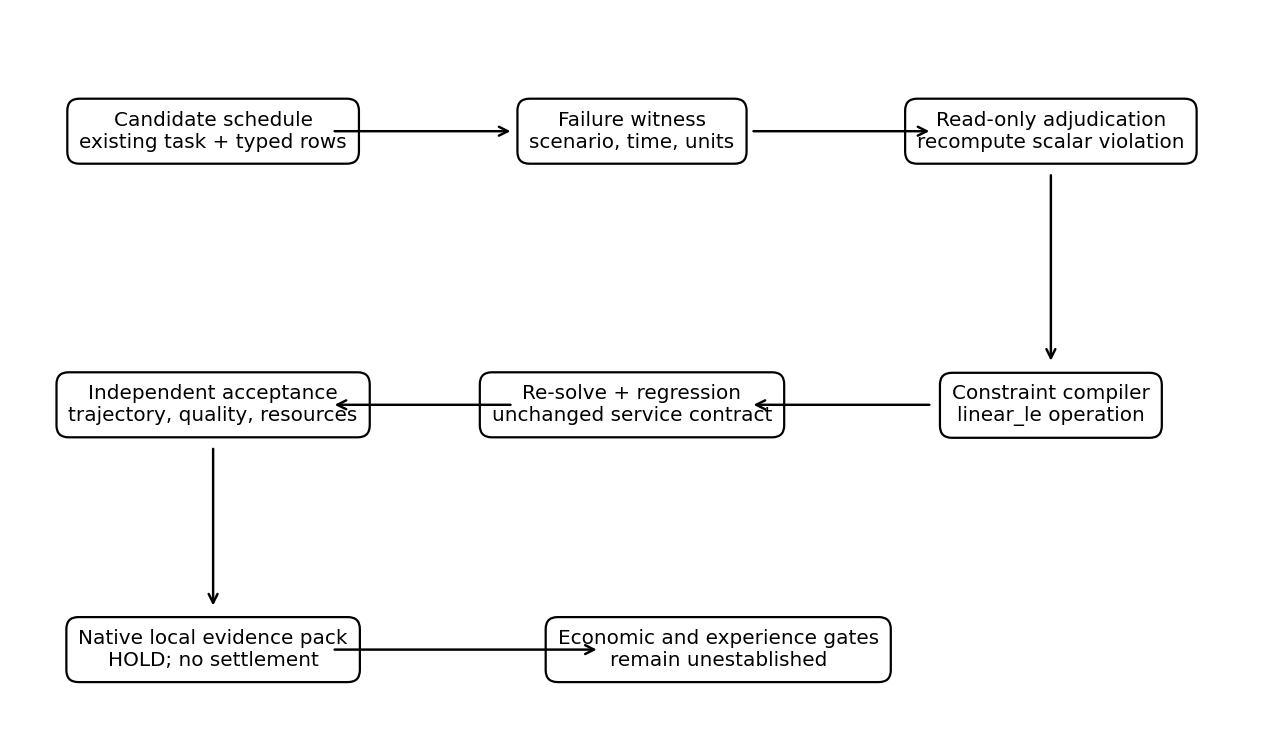
\includegraphics[width=0.96\textwidth,height=\textheight]{figures/mechanism.png}
\caption{Implemented evidence flow. Only the upper repair loop and local
pack production are executed as new mechanisms. Economic and
progressive-experience gates remain open; an arrow does not establish
their success.}\label{fig-mechanism}
\end{figure}

\subsection{Typed operational model}\label{typed-operational-model}

Each task specifies a horizon \(T=48\), five supplied scenarios, an
initial stock, a reserve trajectory, a capacity, conversion factors,
losses, power caps, and optionally a ramp limit. The state unit is cubic
metres for water, thermal kilowatt-hours for industrial heat, or
kilowatt-hours for charging. These are three unit-labelled model domains
with the same scalar recurrence, not three separately validated physical
industries.

For scenario \(k\) and time \(t\),

\[
x_{k,t+1}=a_{k,t}x_{k,t}+\Delta t\bigl(\eta_{k,t}u_t-d_{k,t}\bigr),\qquad
\ell_{t+1}\leq x_{k,t+1}\leq U.
\]

Here \(a\) is dimensionless retention, \(u\) is power in kW,
\(\Delta t\) is hours, \(\eta\) converts electrical energy to the
declared stock unit, and \(d\) is stock consumed per hour. The objective
maximizes a common event-period reduction \(r\), subject to power and
ramp constraints. The same dispatch \(u\) must serve all declared
scenarios. The oracle measures the optimum of this finite linear model,
not statistical or physical reliability beyond it.

The structural map preserves conservation-like accumulation, loss,
supply, and demand relationships. Units are explicit. Applicability
requires the supplied linear dynamics and constraints. Nonlinear
equipment behavior, hidden shared limits, unmodeled failures, changing
prices, and actual operating obligations lie outside the claim. The
mapping itself was supplied by the task designer; no autonomous search
discovered that these physical domains share a recurrence.

\subsection{Witness to executable
inequality}\label{witness-to-executable-inequality}

The starting candidate includes all power/ramp requirements and the
inventory constraints for scenario zero. This is a deliberately
incomplete candidate for studying repair; it is \textbf{not} the
strongest baseline. All scenarios are available to every arm, and the
complete LP uses them directly.

The critic finds the first violated inventory bound, scanning scenarios
and then time. The witness contains the task hash, scenario index, time
index, state unit, observed stock, required bound, and prefix length.
``Minimal'' here means the shortest violating prefix in the first
selected scenario. The implementation does not establish global
minimality across all scenarios or a minimal explanation among arbitrary
causal descriptions.

The adjudicator independently recomputes that scalar prefix from the
unchanged task and candidate. Wrong units, mismatched identity,
malformed indices, nonfinite values, and unreproduced claims are
rejected. A valid witness is converted to a \texttt{linear\_le}
operation. Writing

\[
A_{k,t}=\prod_{h=0}^{t}a_{k,h},\qquad
b_{k,t}=A_{k,t}x_0-\Delta t\sum_{j=0}^{t}d_{k,j}\prod_{h=j+1}^{t}a_{k,h},
\]

and

\[
w_{k,t,j}=\Delta t\,\eta_{k,j}\prod_{h=j+1}^{t}a_{k,h},
\]

\Needspace{7\baselineskip}

The lower-stock obligation becomes

\[
-\sum_{j=0}^{t}w_{k,t,j}u_j\leq b_{k,t}-\ell_{t+1}.
\]

The upper-stock obligation uses the opposite coefficient sign and
\(U-b_{k,t}\). Empty products equal one. The coefficients have
stock-unit/kW dimensions; the right-hand side has stock units. These
rows are consequences of the original service contract, not a relaxed
replacement for it. The final model may not change market parameters or
the acceptance judge to make a repair pass.

The interpreter permits only task-bound \texttt{linear\_le} operations
of the declared shape. Generated operations cannot invoke a shell,
network, hardware, or real transaction. The development process's
authorized tools are distinct from generated-strategy capabilities. A
maximum of 128 new cuts and a two-second candidate CPU limit bound each
attempt; final resource acceptance also observes worker CPU externally.
The common final checker retains the 0.999 useful-quality floor and the
inherited abstract-work ceiling.

\subsection{An actual counterexample-to-adaptation
trace}\label{an-actual-counterexample-to-adaptation-trace}

The retained task \texttt{writer-exploratory-0796104bb23547932bef}, seed
89110, is the industrial-thermal/shared-linear case. Its capacity is
1,476.643381 thermal kWh and initial stock 959.818198 thermal kWh. The
first candidate claims a reduction of \textbf{536.049417 kW}. In
scenario 1, after the fifth step, its stock is \textbf{264.220505
thermal kWh}, below the required \textbf{265.795809}. Independent scalar
recomputation gives a violation of \textbf{1.575304 thermal kWh}.

The compiler produces the concrete additional constraint

\[
\begin{aligned}
-0.907916553u_0-0.910922454u_1-0.913938307u_2\\
-0.916964144u_3-0.920000000u_4\leq-1485.227448635.
\end{aligned}
\]

This row is not a verbal recommendation. It enters the next optimization
call. Fourteen validated additions lead to a reduction of
\textbf{515.076648 kW}, matching the independent finite-model optimum.
The direct trajectory checker reports a maximum numerical bound
violation of approximately \(4.6\times10^{-12}\) stock units, below its
declared tolerance. The complete before schedules, witness,
adjudication, row coefficients, final schedule, and native pack are
preserved; Appendix C gives the exact record path.

The causal improvement is from an invalid partial-model schedule to a
valid complete-contract schedule. It is not an improvement over the full
LP, which starts with the relevant constraints and returns the same
optimum. Nor does the row by itself constitute reusable domain-general
knowledge: it is bound to one task's parameters. A reusable compiler is
an engineered tool; a learned strategy that improves how future tools
are invented would need a different experiment.

\begin{longtable}[]{@{}
  >{\raggedright\arraybackslash}p{(\columnwidth - 4\tabcolsep) * \real{0.3333}}
  >{\raggedright\arraybackslash}p{(\columnwidth - 4\tabcolsep) * \real{0.3333}}
  >{\raggedright\arraybackslash}p{(\columnwidth - 4\tabcolsep) * \real{0.3333}}@{}}
\caption{Attribution of supplied mathematics, engineered code, and
generated artifacts.}\tabularnewline
\toprule\noalign{}
\begin{minipage}[b]{\linewidth}\raggedright
Element
\end{minipage} & \begin{minipage}[b]{\linewidth}\raggedright
Supplied / implemented by writer
\end{minipage} & \begin{minipage}[b]{\linewidth}\raggedright
Generated or verified at runtime
\end{minipage} \\
\midrule\noalign{}
\endfirsthead
\toprule\noalign{}
\begin{minipage}[b]{\linewidth}\raggedright
Element
\end{minipage} & \begin{minipage}[b]{\linewidth}\raggedright
Supplied / implemented by writer
\end{minipage} & \begin{minipage}[b]{\linewidth}\raggedright
Generated or verified at runtime
\end{minipage} \\
\midrule\noalign{}
\endhead
\bottomrule\noalign{}
\endlastfoot
Task and analogy & Known scalar recurrence; three unit-labelled model
domains & No autonomous analogy discovery \\
Construction grammar & Task-bound linear inequalities and bounded solve
loop & Scenario/time-specific numerical rows and schedules \\
Criticism & Inventory-bound witness search and scalar adjudicator &
Reproduced failures; wrong-unit criticisms rejected \\
Acceptance & Unchanged direct checker and separate optimum formulation &
Original-contract quality/resource verdict \\
Economic / physical instruments & No new sensor, reagent, purchase or
customer contract & No new physical or commercial result \\
Cumulative invention & No cross-task learner in the new pilot &
Task-specific rows are not claimed as transferable learning \\
\end{longtable}

\section{Frozen exploratory pilots and verification}\label{methods}

\subsection{Why a targeted pilot, not another expensive
factorial}\label{why-a-targeted-pilot-not-another-expensive-factorial}

The developer already attempted a full eight-arm A/S/C comparison, but
the missing constructive feedback edge made a new broad factorial
premature. We instead test the narrow causal mechanism before any
business or general-intelligence claim. The four arms are the complete
conventional LP; a scenario-zero partial model with no constructive
correction; the same partial model exposed to a deliberately wrong-unit
criticism; and the validated corrective loop.

The two incomplete arms are \textbf{mechanism ablations}, not
competitive service alternatives. Their purpose is to test whether the
new edge changes the artifact and whether unvalidated criticism is
refused. Their failure cannot establish superiority over competent
ordinary methods. The full LP remains the primary useful comparator. All
arms have the same current-task information, allowed solvers, resource
ceilings, and final acceptance checks; they differ in whether and how
constraints are constructed.

Each panel contains 36 task identities: three seeds, three unit-labelled
domains, and four structures---shared linear dynamics, ramp coupling,
scenario-dependent loss, and time-varying parameters. Horizon and
scenario count are fixed. Arm order is randomized by a recorded
deterministic ordering seed. The panel is a finite component test, not a
sampled customer population. Domain labels do not make mathematically
related tasks independent scientific domains.

The protocol and source hashes are written before evaluation begins.
Version 2's record is timestamped \textbf{2026-10-29T12:37:43Z} and
declares the scope \textbf{EXPLORATORY}. It explicitly leaves the
minimum economic gain unset because no admitted economic activity
exists. There is no model-weight training or history update. No
final-panel answer enters learning memory. These measures preserve the
bounded test, but the earlier campaign's complete sequential error
ledger was not recovered; changing versions cannot create new
confirmatory permission.

\subsection{First version: correctness was not
enough}\label{first-version-correctness-was-not-enough}

The first fixed panel used base seeds 70101, 70202, and 70303. The
corrective procedure accepted 33 of 36 tasks; three repairs exceeded the
unchanged CPU gate. All 36 complete-LP tasks passed. The first tool call
terminated after 75 records. We verified no controller remained active
and completed the 69 predeclared missing records in recorded segments
without changing candidate or checker code. Original records and
interruption metadata were preserved. Some aggregate controller costs
could not be reconstructed completely, so we do not present a complete
monetary cost for this segmented run.

The diagnosed overhead included recalculating an invariant task digest
for every stored constraint on each solve. A versioned repair hoisted
that calculation outside the row-validation loop. It did not remove
identity checks, alter constraints, loosen tolerances, change the
two-second ceiling, or edit the final evaluator. The first version's
source snapshot and failed results remain available and retired as
exploratory development evidence.

\subsection{Second version: fresh tasks, same
acceptance}\label{second-version-fresh-tasks-same-acceptance}

The second panel used fresh base seeds 88101, 88202, and 88303. All 144
arm/task records completed in one block. Parent and child CPU were
measured, native workbench overhead was recorded, and saved artifact
digests were retained. The reported wall time is 23.053901 seconds;
parent CPU is 2.007817 seconds and children CPU 21.201086 seconds. Peak
child resident memory reported by the operating system was 126,576 KiB.
These are run measurements, not the total cost of designing,
researching, writing, verifying, and packaging the campaign.

Because versions use different task panels and execution histories, the
change in their measured CPU is not a randomized causal speedup estimate
for the digest optimization. The defensible observations are that the
identified redundant work was removed, the next frozen version passed
the resource gate on all fresh cases, and the conventional reference
remained cheaper. No holdout was repeatedly tuned until success.

\subsection{What independent checking actually
checked}\label{what-independent-checking-actually-checked}

The original study's 71 tests, the original Omega laboratory's 51 tests,
the first-cycle fixture's five tests, and 14 new corrective tests passed
in this environment. Counts belong to distinct suites, not independent
scientific replications. The new tests exercise compiled rows, witness
rejection, malformed operations, wrong units, and unchanged obligations.
No test was weakened to turn a preferred result green.

After both panels, read-only native inspection reproduced all
\textbf{288} pack/binding and final-acceptance records. A separate
coefficient audit validated \textbf{626} generated additions in version
1 and \textbf{594} in version 2, using a closed-product calculation
rather than the builder's forward recurrence. It recomputed 72
finite-model optima and checked all 72 deliberately invalid-criticism
rejections. The unchanged original source and the version-2 freeze
hashes were also checked. This is strong evidence of the specific local
mechanism, not an external safety certification or proof against every
numerical library defect.

\section{Technical results: repair succeeds, the baseline still
wins}\label{technical-results}

\begin{longtable}[]{@{}lllll@{}}
\caption{New raw-record reaggregation. Both panels retain every
attempted task. CPU is an all-record deployment proxy, not complete
monetary cost. The complete LP is the primary competent
comparator.}\tabularnewline
\toprule\noalign{}
Arm & v1 accepted & v2 accepted & v2 new rows & v2 CPU/attempt (s) \\
\midrule\noalign{}
\endfirsthead
\toprule\noalign{}
Arm & v1 accepted & v2 accepted & v2 new rows & v2 CPU/attempt (s) \\
\midrule\noalign{}
\endhead
\bottomrule\noalign{}
\endlastfoot
Complete LP & 36/36 & 36/36 & 0 & 0.123720 \\
Partial-model selection & 0/36 & 0/36 & 0 & 0.125518 \\
Invalid-criticism control & 0/36 & 0/36 & 0 & 0.125890 \\
Verified correction & 33/36 & 36/36 & 594 & 0.239909 \\
\end{longtable}

Both complete LP and corrective construction pass every task in the
revised panel. Each has 12/12 accepted cases in each unit-labelled
domain. The two incomplete ablations pass none. Every wrong-unit
criticism is rejected, and therefore cannot silently become an
executable constraint. That control establishes evidence gating, not an
ability to recognize all forms of irrelevant criticism.

The corrective arm constructs 594 new rows across 36 tasks. Its accepted
normalized quality has a minimum within approximately
\(2.1\times10^{-15}\) of one. The useful comparison is thus a tie in
finite-model quality. The construction is more expensive: its deployment
CPU proxy per attempted task is \textbf{0.239909 seconds}, versus
\textbf{0.123720 seconds} for the complete LP. This proxy adds observed
worker CPU, native-process CPU, and allocated evaluation-oracle CPU.
Candidate self-reported CPU is a subset and is not added again. All
failed attempts remain in the totals.

\begin{figure}
\centering
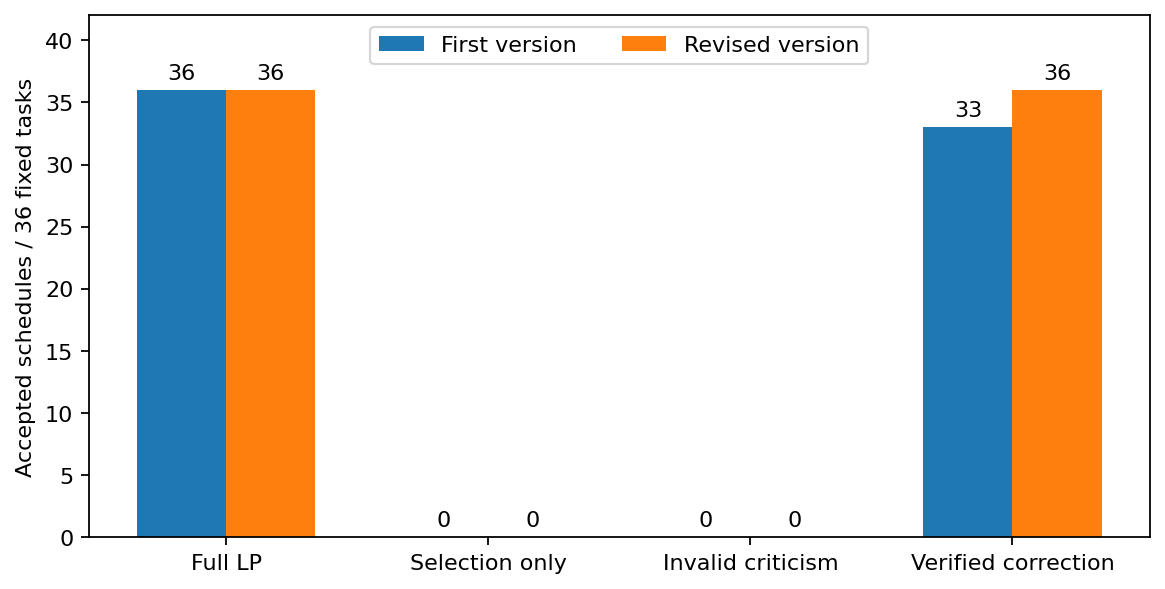
\includegraphics[width=0.9\textwidth,height=\textheight]{figures/acceptance.png}
\caption{Accepted schedules in both frozen exploratory panels. The first
version's three resource failures are retained. The conventional LP
succeeds on both panels; the repaired mechanism does not exceed
it.}\label{fig-acceptance}
\end{figure}

\begin{figure}
\centering
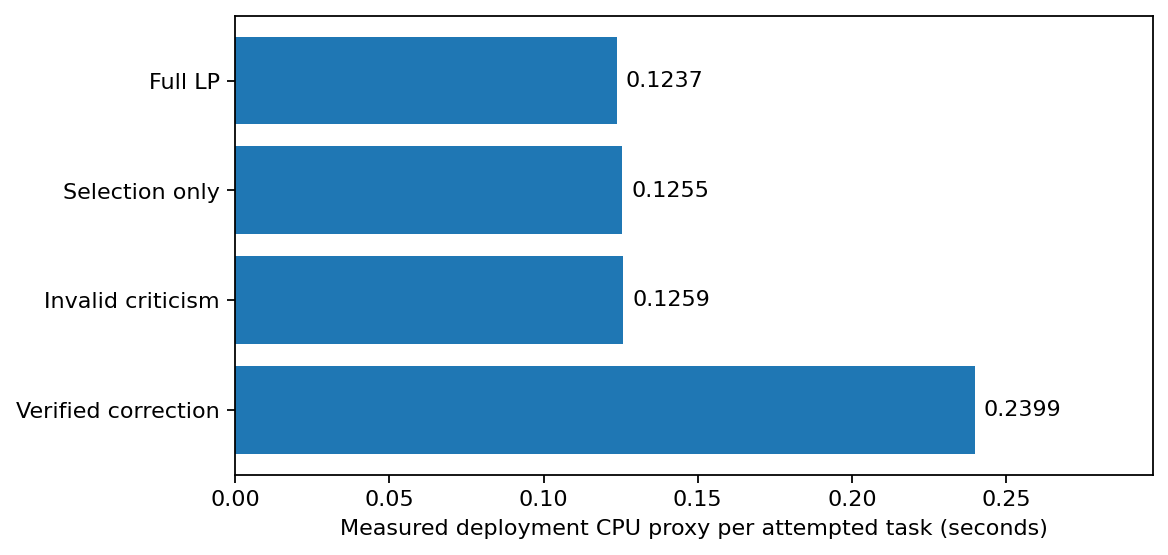
\includegraphics[width=0.92\textwidth,height=\textheight]{figures/cpu.png}
\caption{Revised-panel measured deployment CPU proxy per attempted task.
This is not a provider invoice or full research cost. Incomplete
ablations have no accepted outputs, so their cost per accepted output is
undefined, not zero.}\label{fig-cpu}
\end{figure}

\subsection{No general synergy claim
follows}\label{no-general-synergy-claim-follows}

These results do not test a multiplicative discovery advantage. The
mechanism uses a supplied cross-domain recurrence and a writer-designed
operation language. It performs finite constraint construction, not
open-ended strategy invention. The ablations identify the utility of
constructive feedback relative to an intentionally partial candidate;
they do not isolate independently learned A, S, and C contributions on
consequential business work. The primary competent alternative already
implements the complete mathematical specification.

The appropriate technical decision is therefore \textbf{GO for this
bounded corrective component, HOLD for superior useful capability}. A
component can be correct and useful for engineering the broader system
without being the best production path for its current application.
Retaining the full LP as the preferred route prevents the research
mechanism from degrading delivery merely because it has a more ambitious
name.

\subsection{The preserved eight-arm
result}\label{the-preserved-eight-arm-result}

The inherited A/S/C study reports 144/144 accepted outputs in every arm.
The full combination's mean usefulness is slightly below the complete LP
due to numerical approximation, not substantively above it. Its reported
CPU proxy is 1.099252 seconds per accepted output, versus 0.781836 for
neither mechanism and 0.745085 for the conventional portfolio reference.
Complete numbers are retained in Appendix D (\citeproc{ref-dev}{AGI
ALPHA development record 2026a}).

The declared aggregate interaction contrast was

\[
I=\mu_{111}-\mu_{100}-\mu_{010}-\mu_{001}+2\mu_{000}.
\]

The reported estimate is \(5.00324\times10^{-7}\) with interval
\([2.91796,7.08873]\times10^{-7}\), versus a practical threshold of
0.02. This is a sum-of-interactions contrast on the declared additive
scale, not by itself a pure three-way interaction coefficient and not a
multiplicative effect. Its tiny positive value arises because
overlapping components do not incur the same small approximation error
twice. The combination does not acquire useful superiority by that
arithmetic. We verified the contrast's consistency with the supplied
means; without the raw paired archive, we cannot independently recreate
its confidence interval.

The historical transfer table also preserves 288 applicability-refused
requests across A-enabled arms and 288 valid, quality-neutral transfer
requests. A refusal is not a harmful delivered transfer; an accepted
fallback can still solve the task. No inference about real-world
transfer rates follows from the fixture mixture. The new edition does
not relabel those old outcomes as new evidence.

\section{Experience: distinguish retained assets from improved
invention}\label{experience}

A library can grow while usefulness does not. A previously checked
artifact may lower the cost of one later operation; that is productive
reuse. A genuine compounding claim is stronger: accumulated experience
must causally improve the process of discovering or constructing future
useful capabilities after acquisition, retrieval, adaptation,
maintenance, and verification costs.

The recovered original compounding summaries compare cumulative, frozen,
reset, and ordinary-retrieval modes. The final panel reports 72 accepted
outputs for every mode. Cumulative mean deployment CPU is 1.309692
seconds, versus 1.351033 frozen, 1.368085 reset, and 1.378608 retrieval.
The reported paired differences favor cumulative in point estimate, but
every interval crosses zero. Reset and frozen are also closely related
implementations of the same fixed policy in a largely stateless task
setting, which limits the breadth of the comparison
(\citeproc{ref-dev}{AGI ALPHA development record 2026a}).

\begin{longtable}[]{@{}
  >{\raggedright\arraybackslash}p{(\columnwidth - 6\tabcolsep) * \real{0.2500}}
  >{\raggedright\arraybackslash}p{(\columnwidth - 6\tabcolsep) * \real{0.2500}}
  >{\raggedright\arraybackslash}p{(\columnwidth - 6\tabcolsep) * \real{0.2500}}
  >{\raggedright\arraybackslash}p{(\columnwidth - 6\tabcolsep) * \real{0.2500}}@{}}
\caption{Inherited final-panel comparison. Twenty-four reported pairing
clusters; interval computation not independently reproduced because raw
pairs are missing.}\tabularnewline
\toprule\noalign{}
\begin{minipage}[b]{\linewidth}\raggedright
Control − cumulative
\end{minipage} & \begin{minipage}[b]{\linewidth}\raggedright
Reported saving (s)
\end{minipage} & \begin{minipage}[b]{\linewidth}\raggedright
Reported interval (s)
\end{minipage} & \begin{minipage}[b]{\linewidth}\raggedright
Decision
\end{minipage} \\
\midrule\noalign{}
\endfirsthead
\toprule\noalign{}
\begin{minipage}[b]{\linewidth}\raggedright
Control − cumulative
\end{minipage} & \begin{minipage}[b]{\linewidth}\raggedright
Reported saving (s)
\end{minipage} & \begin{minipage}[b]{\linewidth}\raggedright
Reported interval (s)
\end{minipage} & \begin{minipage}[b]{\linewidth}\raggedright
Decision
\end{minipage} \\
\midrule\noalign{}
\endhead
\bottomrule\noalign{}
\endlastfoot
frozen & 0.041341 & {[}-0.084110, 0.153907{]} & Includes zero \\
reset & 0.058394 & {[}-0.072706, 0.185644{]} & Includes zero \\
retrieval & 0.068916 & {[}-0.031334, 0.161136{]} & Includes zero \\
\end{longtable}

\begin{figure}
\centering
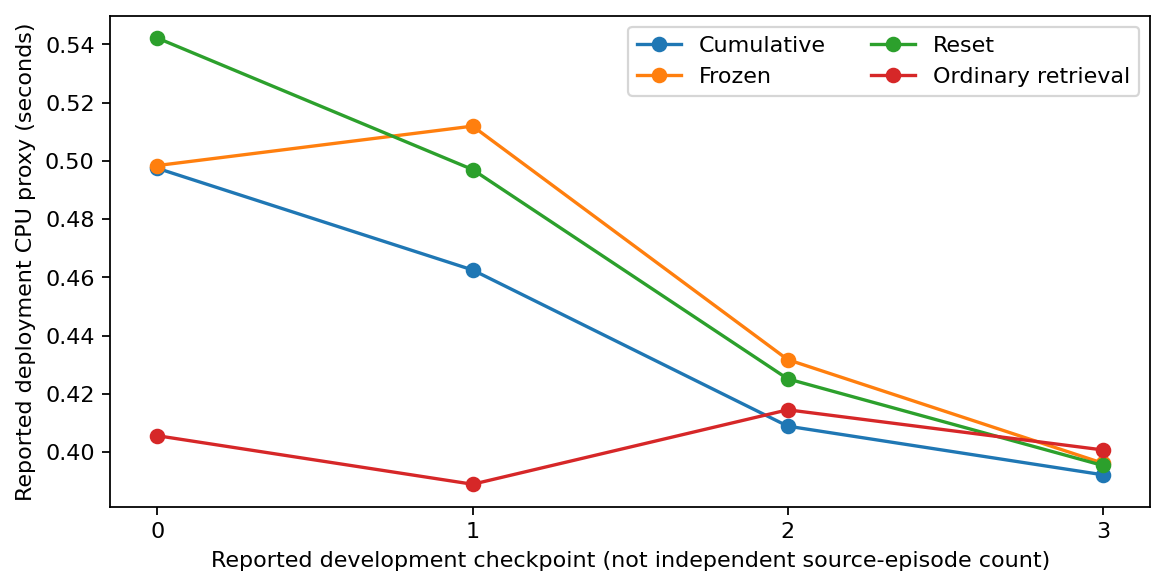
\includegraphics[width=0.92\textwidth,height=\textheight]{figures/historical-learning.png}
\caption{Historical checkpoint trajectory reconstructed from the
supplied aggregate CSV, not from recovered raw tasks. Declining CPU is
also observed in controls. Checkpoint numbers do not certify independent
source episodes or a learned improvement.}\label{fig-history}
\end{figure}

\begin{figure}
\centering
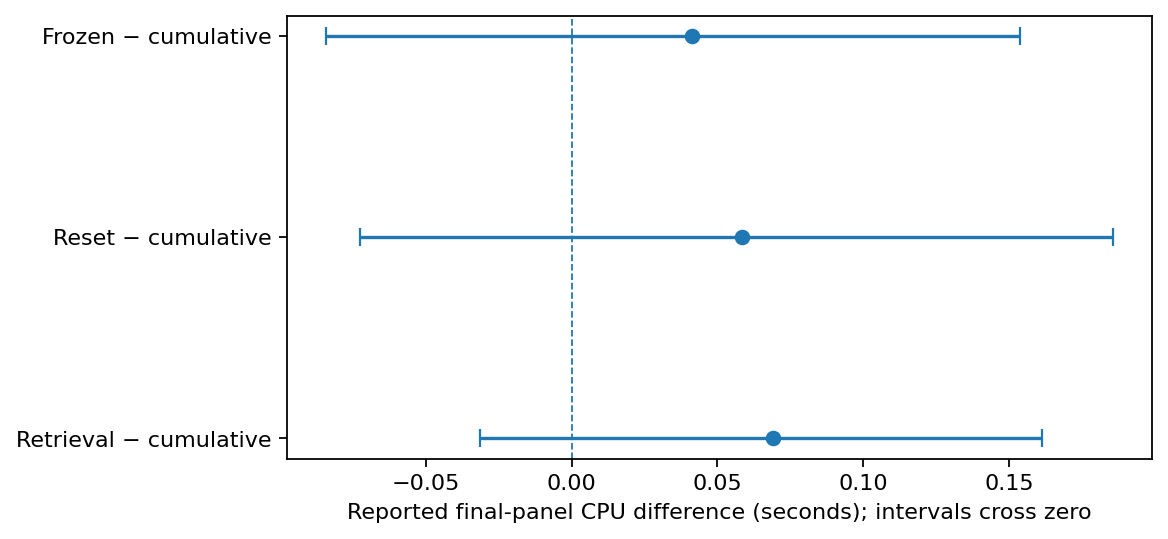
\includegraphics[width=0.92\textwidth,height=\textheight]{figures/historical-intervals.png}
\caption{Reported final-panel differences between each control and the
cumulative mode. The raw paired archive is unavailable in this edition,
so the supplied uncertainty intervals are attributed rather than
independently recomputed. Every interval includes
zero.}\label{fig-intervals}
\end{figure}

Lifecycle accounting changes the interpretation again. Summing the three
reported learning streams gives cumulative deployment/acquisition CPU of
\textbf{179.500251}, frozen \textbf{170.047891}, reset
\textbf{172.048264}, and ordinary retrieval \textbf{179.017008} seconds
under their stated acquisition rules. A sensitivity that charges all
modes for collecting the same later history is separately retained.
Neither accounting convention can turn an uncertain deployment
comparison into a demonstrated better invention process. These are CPU
proxies; model authoring and campaign costs are not monetized
completely.

The new corrective pilot deliberately has no cross-task memory. Its 594
rows are task-bound constraints, not 594 learned transferable scientific
principles. The reusable compiler was engineered in this session; there
is no causal comparison showing that earlier generated rows made later
invention cheaper or more successful. No new ``0, 4, 8, 12 episodes''
table is fabricated. \textbf{Experience GO remains unestablished.}

A future admissible learning test would retain the failure
\emph{family}, its applicability assumptions, the transformation rule,
and measured costs, not reuse a previous final schedule under a new
identifier. Current inputs, strong tools, task difficulty, and total
budgets would remain comparable across cumulative and ordinary-retrieval
controls. Such a test is a continuation requirement, not a result of
this paper.

\section{Economic audit: a profitable checkpoint was not a profitable
campaign}\label{economics}

\subsection{The evidence that can be
audited}\label{the-evidence-that-can-be-audited}

The structural-transfer package contains more than a report: task
artifacts, saved checkers, simulated receipts, expense events,
investment records, and SQLite histories. Its five technical arms each
produce 24 accepted certificates: four feasible schedules and twenty
infeasibility certificates. An accepted infeasibility certificate is a
valid analytical output, not a completed feasible operation. Across all
120 primary certificates and eight successor certificates, the saved
checker succeeds. There is no accepted-output advantage for the
instrument over ordinary reuse, target specialist, coded generalist
reference, or enterprise without the instrument
(\citeproc{ref-transfer}{AGI ALPHA development record 2026c}).

The ``frontier generalist'' label in that package does not mean a live
frontier model solved each case. The implementation includes a coded
comparator and an authoring-token allowance. We preserve its actual
identity rather than treating its name as a defeated AI competitor.
Physical delivery and real market demand were not observed.

\subsection{Reconciliation from the latest database, not a stale
report}\label{reconciliation-from-the-latest-database-not-a-stale-report}

The earlier instrument snapshot showed 9.200000 SIM USD revenue,
8.656447 expense, and \textbf{+0.543553} operating profit. Late
post-gate regression, documentation, audit, writer-allowance, and
retention expenses added \textbf{7.118500}, changing profit to
\textbf{−6.574947}. A subsequent developer budget-repair receipt added
\textbf{2.000000}, producing the current \textbf{−8.574947}. These
historical snapshots remain unchanged and separately hashed.

The writer's first replay compared the current database with the older
cost-reconciliation snapshot and failed its expected-value checks.
Inspection found the already-recorded later repair receipt. We did not
erase or ``fix'' the database to recover the positive figure; we
replayed the read-only auditor against the latest versioned receipt.
Instrument, control, and full-refund snapshots then all reconciled. The
initial failed audit is retained as evidence of a source-version
mismatch, not concealed as a successful first attempt.

\begin{longtable}[]{@{}llll@{}}
\caption{Versioned instrument cost bridge, SIM USD. No prices or demand
were improved to repair the result.}\tabularnewline
\toprule\noalign{}
Recorded stage & Revenue & Expense & Profit \\
\midrule\noalign{}
\endfirsthead
\toprule\noalign{}
Recorded stage & Revenue & Expense & Profit \\
\midrule\noalign{}
\endhead
\bottomrule\noalign{}
\endlastfoot
Earlier positive checkpoint & 9.200000 & 8.656447 & 0.543553 \\
Late-cost reconciliation & 9.200000 & 15.774947 & -6.574947 \\
Later seed-repair receipt & 9.200000 & 17.774947 & -8.574947 \\
\end{longtable}

\begin{figure}
\centering
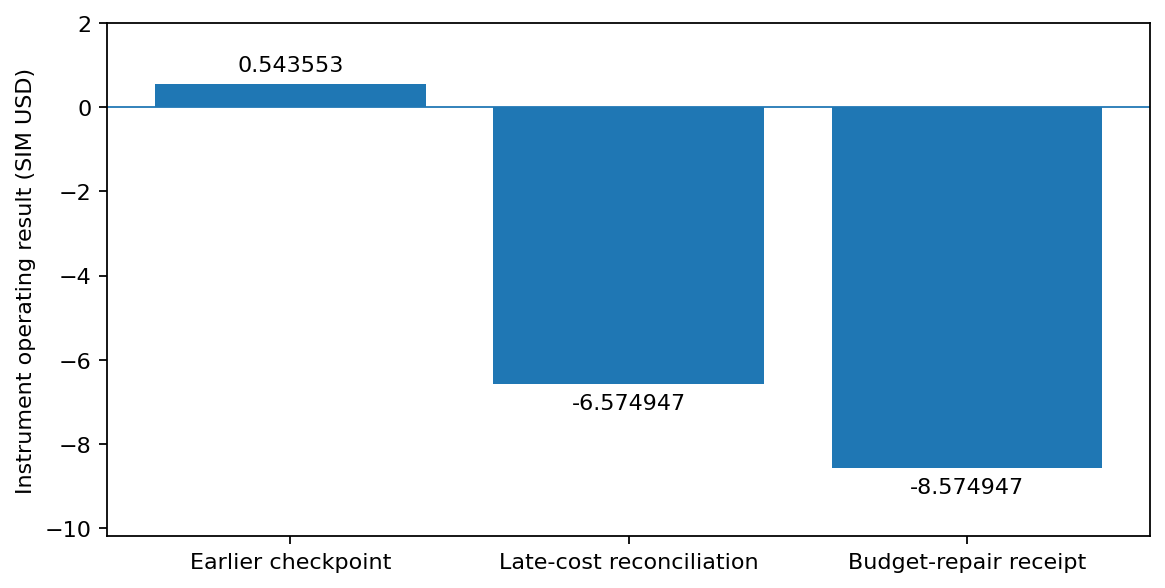
\includegraphics[width=0.94\textwidth,height=\textheight]{figures/profit-bridge.png}
\caption{The instrument's before-and-after cost bridge. Revenue stays
fixed while previously omitted and later repair expenses are recognized.
These are SIM accounting snapshots, not realized currency receipts or a
newly observed market.}\label{fig-profit}
\end{figure}

The late expenses include explicit estimates under reference-rate
assumptions rather than metered provider invoices. Deterministic steps
are not assigned fictional language-model calls, but unmetered authoring
and closing work remains estimated. The present writer's additional
research, implementation, checking, and manuscript work is \textbf{not}
silently inserted into the earlier developer's ledger, and is not zero.
Its measured local resources are recorded separately; exact inference
cost is unknown. Consequently the ledger's loss is an auditable recorded
scenario result, not a complete externally validated economic
measurement of every resource consumed across conversations.

\subsection{Profit, cash, reserves, and payback are different
quantities}\label{profit-cash-reserves-and-payback-are-different-quantities}

The latest instrument database contains revenue \textbf{9.200000},
expenses \textbf{17.774947}, profit \textbf{−8.574947}, cash
\textbf{30.304453}, a tail reserve of \textbf{18.400000}, and working
capital of \textbf{1.000000}, all in SIM USD. Available cash after those
restrictions is \textbf{10.904453}. \textbf{Unrestricted earned funds
are zero.} Cash remains because financing capital is present; cash
remaining is not evidence of profit.

The funded control has revenue \textbf{11.000000}, recorded expenses
\textbf{10.604113}, and operating profit \textbf{+0.395887}. Its larger
remaining cash is not a matched claim of a real profitable customer
business. Its wider project still carries unrecovered research costs,
and its simulated offering is not the newly screened cohort. The
instrument's explicitly recorded cumulative project result is
\textbf{−40.304617}, including separately identified inherited research
and seed costs without charging them again per delivery.

\begin{longtable}[]{@{}
  >{\raggedright\arraybackslash}p{(\columnwidth - 6\tabcolsep) * \real{0.2500}}
  >{\raggedright\arraybackslash}p{(\columnwidth - 6\tabcolsep) * \real{0.2500}}
  >{\raggedright\arraybackslash}p{(\columnwidth - 6\tabcolsep) * \real{0.2500}}
  >{\raggedright\arraybackslash}p{(\columnwidth - 6\tabcolsep) * \real{0.2500}}@{}}
\caption{Read-only latest-snapshot reconciliation, SIM USD. Financing
capital and reserves are not revenue.}\tabularnewline
\toprule\noalign{}
\begin{minipage}[b]{\linewidth}\raggedright
Latest audited quantity
\end{minipage} & \begin{minipage}[b]{\linewidth}\raggedright
Instrument
\end{minipage} & \begin{minipage}[b]{\linewidth}\raggedright
Funded control
\end{minipage} & \begin{minipage}[b]{\linewidth}\raggedright
Instrument refund branch
\end{minipage} \\
\midrule\noalign{}
\endfirsthead
\toprule\noalign{}
\begin{minipage}[b]{\linewidth}\raggedright
Latest audited quantity
\end{minipage} & \begin{minipage}[b]{\linewidth}\raggedright
Instrument
\end{minipage} & \begin{minipage}[b]{\linewidth}\raggedright
Funded control
\end{minipage} & \begin{minipage}[b]{\linewidth}\raggedright
Instrument refund branch
\end{minipage} \\
\midrule\noalign{}
\endhead
\bottomrule\noalign{}
\endlastfoot
Earned SIM revenue & 9.200000 & 11.000000 & 0.000000 \\
Recorded expenses & 17.774947 & 10.604113 & 26.974947 \\
Operating profit & -8.574947 & 0.395887 & -26.974947 \\
Cash & 30.304453 & 49.628387 & 11.904453 \\
Tail reserve & 18.400000 & 22.000000 & 0.000000 \\
Working capital & 1.000000 & 1.000000 & 1.000000 \\
Available cash & 10.904453 & 26.628387 & 10.904453 \\
Unrestricted earned & 0.000000 & 0.395887 & 0.000000 \\
\end{longtable}

\begin{figure}
\centering
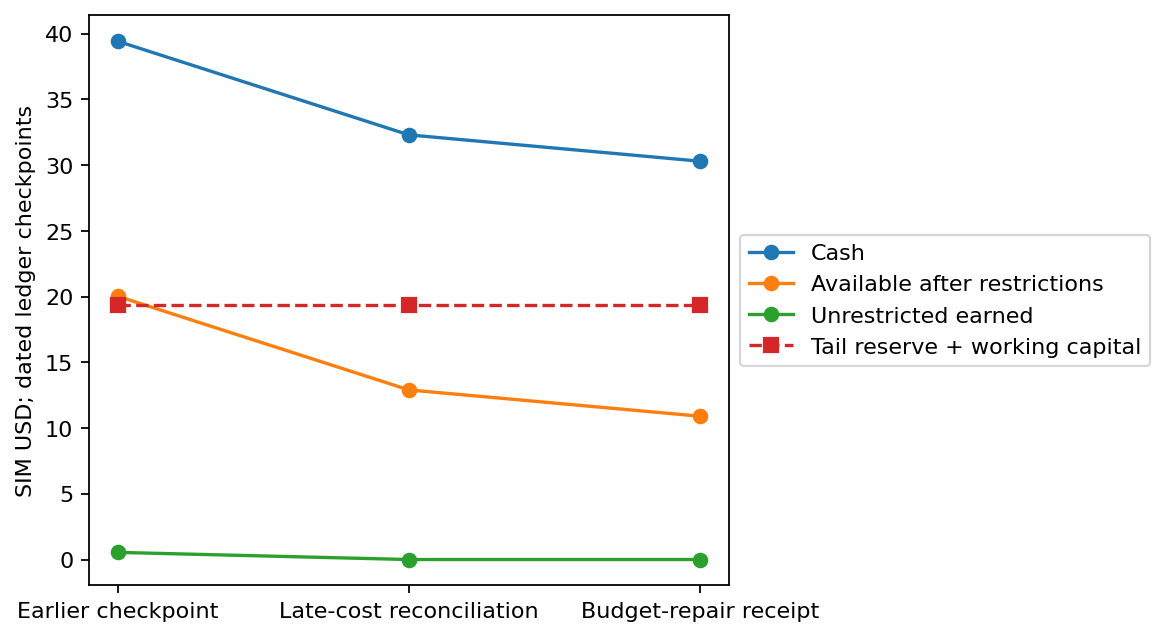
\includegraphics[width=0.96\textwidth,height=\textheight]{figures/cash.png}
\caption{Cash, restrictions, and earned funds across the instrument's
actual recorded reconciliation sequence. The horizontal positions are
ordered ledger checkpoints, not equally spaced operating periods.
Remaining financed cash must not be described as earned
surplus.}\label{fig-cash}
\end{figure}

The protected simulator recognizes reserved commitments before computing
free funds. The read-only audit checks exact integer accounting,
expense-payment bounds, receipt/event consistency, provider-binding
fields, historical investment reservations, and wallet conservation. Its
signature checks use the local simulation provider's assumptions; they
do not establish an independent external payment provider or real
finality. No actual wallet, key, payment, token trade, or native
transaction was accessed or authorized.

\subsection{No identified negative-to-positive
crossing}\label{no-identified-negative-to-positive-crossing}

A transformation claim would require the same admitted cohort to have a
credible negative complete-cost baseline and a positive complete-cost
treatment, caused by the constructed instrument. The recovered evidence
shows neither. In the transferable scheduling study the strong
comparator already solves the model. In the structural-transfer market,
the instrument has a worse recorded operating result than the funded
control. In the three real-world prospects, the cohort and cost/value
bridge remain unestablished.

Nor do the 216 refusal worlds in the original compounding source
establish a market. They exercise a qualification/refusal gate, with
zero orders, not measured demand and competitive customer selection. A
zero result in that fixture does not identify the market value of a
physically validated future instrument. Conversely, predicted customer
benefit is not AGI ALPHA license revenue, token demand, or ownership
value.

We do not report NPV because the required coherent cash-flow horizon,
investment alternatives, financing convention, and calibrated
uncertainty are not available for a real admitted cohort. We also do not
double-count capital outlay and depreciation or reserve transfers and
the underlying obligation. Profit, payback, liquidity, investment
attractiveness, and value capture remain separate decisions.

\section{Protected exchange and the successor link}\label{successor}

The recovered simulation traces offer, inspection, acceptance, receipts,
refunds, liabilities, and reserved investment. Its current instrument
history has 46 simulated orders, 333 events, and one investment record.
The control has 55 orders, 392 events, and one investment record. These
are generated exchange histories under declared rules, not customer
observations. A sufficiently equivalent free completed service is a
legitimate adverse alternative, but the package's exact-free-output case
is a sensitivity scenario, not proof that such a current service exists.

A historical 0.25-SIM-USD investment event can remain a genuine
chronological event in the simulator even after subsequent lifecycle
accounting reverses the apparent surplus. The correct response is not to
delete the event or to call the entire subsequent construction free. It
is to ask which funds were available at the decision, which costs were
omitted or later incurred, and whether the completed successor produced
an incremental return that covers its construction and lifecycle
obligations.

The saved successor comparison has four fresh pairs. Both instrument and
funded no-instrument control accept all four. The predecessor's exact
interface cannot express the new shared-capacity obligation; two old
relaxed schedules violate it. Thus a meaningful new interface capability
was constructed relative to that restricted predecessor, but the
competent funded control also constructs it. The attributable
accepted-output advantage is \textbf{zero}. This is precisely why ``new
compared with old code'' is not equivalent to ``caused by the proposed
transfer engine.''

The instrument's recorded successor feature net return after its
reported lifecycle charges is \textbf{−6.832946 SIM USD}; the control's
is \textbf{−0.217140}. The later 2.00 budget-repair expense is
explicitly assigned to seed repair, not to that successor feature, and
is not subtracted from the feature twice. Current unrestricted earned
funds in the instrument account remain zero. A full-refund branch yields
profit \textbf{−26.974947}, cash \textbf{11.904453}, and investment
stopped, while preserving construction expenses already incurred.

The new writer corrective compiler is \textbf{not} claimed to have been
financed by those SIM earnings. It was constructed with the existing
authorized local tools and zero new external spending. Its measured
compute and unmetered authoring costs belong to the writer continuation
record. An archive, a prompt, an activated existing tool, or a higher
capital variable would not satisfy earned construction; neither does
this unfunded-by-earnings component repair establish that link
retroactively.

\section{Related mechanisms and the boundary of
analogy}\label{related-work}

Cross-domain transfer can be valuable when a relationship, invariant,
observation, or construction method survives a change of domain. The
scientific obligation is to identify the preserved structure and the
assumptions that do not transfer. Merely relabelling the same recurrence
as water, heat, and charging is not evidence of an intelligence
autonomously discovering an unexpected analogy.

Counterexample-guided synthesis and sketching already connect proposed
programs, specifications, and verification. The inspected Berkeley
source emphasizes supplying high-level structure rather than deriving
every insight from nothing. Our construction is narrower still: it
compiles violated inequalities in a supplied linear family. The distinct
contribution is integration with this repository's mission and evidence
flow and an audited negative comparison, not priority for synthesis or
constraint generation (\citeproc{ref-sketch}{Solar-Lezama 2008}).

Current primary OpenAI materials reinforce the need to distinguish
output, supporting artifacts, and scientific understanding. The October
26 release describes different expert-community review strategies. The
inspected \texttt{openai/math} README states that artifacts come from an
unreleased internal model, have heterogeneous verification status, and
are research data rather than uniformly polished papers. Its
Lean/Comparator instructions describe additional verification tooling;
we inspected those instructions but did not install or run that proof
environment. None of those announcements establishes access to the
proprietary model here or validates our runtime's performance
(\citeproc{ref-openai2026}{OpenAI 2026b},
\citeproc{ref-openaimath}{2026a}).

The practical lesson is not that verification is unnecessary until an
expert can check everything. It is that every claimed transition must
have the right evidence object: a reproduced witness for a defect, an
executable adaptation for a repair, a matched competent comparison for a
capability gain, cohort accounts for an economic crossing, and
chronological funded construction with a fresh control for a flywheel.
One object cannot stand in for all the others.

\section{Limits, failure modes, and retained negative
evidence}\label{limits}

\subsection{What the new experiment cannot
identify}\label{what-the-new-experiment-cannot-identify}

The new models are generated, finite, linear, and known to all arms.
They do not contain real site measurements, chemical uncertainty,
heterogeneous battery histories, physical safety qualification, tariff
negotiation, buyer commitments, or complete lifecycle costs. The quality
ceiling is already reached by the conventional solver. Therefore even
perfect correction cannot establish a new feasible activity in this
model family relative to that solver.

The 36 tasks per version cover a declared finite design, not a
probability sample of productive work. They share a generator and
substantial mathematical structure. We report exact observed counts and
retained records rather than interpreting 36/36 as a universal success
probability. The 594 constraints are not 594 independent discoveries.
The irrelevant-criticism control covers a wrong unit, not every
adversarial or misleading criticism. The implementation's ``minimal
witness'' is prefix-local, not a globally smallest explanation.

The authoring system has pretrained knowledge. A clean task context does
not establish that it has never encountered constraint generation,
energy scheduling, or a relevant analogy. No model weights were trained,
and no live frontier-model baseline was paid for or invoked.
``Autonomous'' applies only to the bounded deterministic execution loop
once the writer-designed program runs, not to unattended business
ownership or general scientific strategy invention.

The generated-row interpreter is a restricted numerical interface, not a
security qualification for arbitrary hostile submitted programs. The
writer supplies the compiler; the pilot checks its emitted rows and
witness units. Some descriptive row metadata are not independently
enforced by the solver interface. The demonstrated trust boundary
therefore covers these generated artifacts, not unrestricted third-party
strategy submissions.

The arms share task information, final acceptance, and candidate
resource ceilings. Their realized orchestration and checking work differ
and are charged in the recorded deployment proxies. This is not a claim
of exact total-lifecycle budget parity: authoring, opportunity research,
and several historical resource quantities remain unmetered. Neither the
acceptance tie nor a descriptive compute comparison establishes a
general discovery-efficiency result.

\subsection{Inference and resource
limitations}\label{inference-and-resource-limitations}

The original 2,184-case archive and its complete error-budget/exposure
ledger are unavailable in this edition. Its aggregate plots and
intervals are inherited claims. The new frozen panels are prospective as
recorded locally, but remain exploratory because there is no recovered
campaign-wide confirmatory allocation, no economic minimum-effect
threshold, and no independently administered hidden-case service.

CPU counters have limited resolution and process scope. Startup,
serialization, orchestration, numerical warm-up, and tool-call
segmentation can affect measured performance. We count the observed
parts without double-counting contained CPU, but do not equate those
totals to a complete invoice. Version 1 has incompletely reconstructed
controller costs. Authoring-model inference, earlier human or AI effort,
and some historic acquisition costs remain unknown. A tight arithmetic
ledger inside SIM does not eliminate uncertainty about the assumptions
used to price or generate its events.

The global eight-hour planning allowance and all preceding consumption
could not be reconstructed from the recovered first-cycle registry. This
continuation does not assume a fresh eight-hour budget. It performed
small replays, two bounded component pilots, source inspection, and
publication preparation while measuring current local use. Additional
storage remained below the supplied two-GiB ceiling, with more than two
GiB free. Verification and publication QA received a separately tracked
allocation. The exact final resource checkpoint accompanies the package;
unknown earlier consumption is retained as unknown.

\subsection{Negative results that remain first-class
artifacts}\label{negative-results-that-remain-first-class-artifacts}

The retained record includes the first version's three CPU refusals; all
72 invalid criticisms; zero accepted partial-model schedules in both
panels; the conventional solver's victories on cost; the original
reported absence of practical A/S/C synergy; the unestablished learning
effect; the stale-financial-snapshot audit failure; the late-cost
reversal of profit; the successor's zero advantage over its funded
control; and the three UNKNOWN opportunity admissions. Earlier developer
failures and snapshots are not overwritten.

A further limitation concerns the series source recovery itself. The
complete canonical enterprise TeX was verified by Git blob, but its
matching foundry companion was not recovered. The \emph{Out-Evolve}
section inputs were not recovered. This limits fresh reproduction of
those prior editions, not compilation of the present standalone paper.
The current source package states the difference instead of quietly
substituting an adjacent manuscript.

\section{Decisions and the next falsifiable
construction}\label{decisions}

\begin{longtable}[]{@{}
  >{\raggedright\arraybackslash}p{(\columnwidth - 4\tabcolsep) * \real{0.3333}}
  >{\raggedright\arraybackslash}p{(\columnwidth - 4\tabcolsep) * \real{0.3333}}
  >{\raggedright\arraybackslash}p{(\columnwidth - 4\tabcolsep) * \real{0.3333}}@{}}
\caption{Separate decisions. Passing document production does not
promote the scientific or commercial mission.}\tabularnewline
\toprule\noalign{}
\begin{minipage}[b]{\linewidth}\raggedright
Decision
\end{minipage} & \begin{minipage}[b]{\linewidth}\raggedright
Current finding
\end{minipage} & \begin{minipage}[b]{\linewidth}\raggedright
Exact missing condition
\end{minipage} \\
\midrule\noalign{}
\endfirsthead
\toprule\noalign{}
\begin{minipage}[b]{\linewidth}\raggedright
Decision
\end{minipage} & \begin{minipage}[b]{\linewidth}\raggedright
Current finding
\end{minipage} & \begin{minipage}[b]{\linewidth}\raggedright
Exact missing condition
\end{minipage} \\
\midrule\noalign{}
\endhead
\bottomrule\noalign{}
\endlastfoot
Technical component & GO, bounded compiler; 36/36 in v2 & Not superior
capability: full LP matches at lower measured compute \\
Commercial profitability & Not established; recorded instrument SIM loss
& Calibrated same-cohort complete-cost positive profit \\
Transformational Blue Sky & NOT ESTABLISHED & Verified technical cause
and negative-to-positive crossing on the same cohort \\
Investment & HOLD for current instrument earned funds & Unrestricted
settled surplus, feasible additional build, justified outside-option
comparison \\
Experience & NOT ESTABLISHED & Fresh causal invention benefit after
acquisition/reuse costs \\
AGI ALPHA value capture & UNKNOWN & Evidence of willingness to pay and a
valid captured-value route \\
Full flywheel & NOT COMPLETE & All preceding links plus useful fresh
successor advantage \\
\end{longtable}

The mission remains \textbf{NOT COMPLETE}. What now exists is an
additive, tested corrective-constraint compiler and a more accurate
source/economic record. Its strongest demonstrated utility is that a
verified defect changes an executable artifact while the original
acceptance requirements remain intact. The strongest conventional
comparator still solves the tested work with lower observed compute.

The next substantive campaign needs an admitted activity whose loss
driver is not already removed by the competent baseline. For battery
reuse, that could require a specified asset cohort and validated
diagnostic or routing intervention; for textiles, measured
difficult-feedstock observability and accepted recovery; for buildings,
current all-in delivery obligations and an independently measured
reduction in a binding transaction or execution cost. These are
alternatives to investigate, not prescribed winners. Missing data or
physical authority should stop their dependent claims, not erase the
executable work already completed.

Within any selected opportunity, the next falsifiable test is a paired
comparison of the actual new instrument with the best complete existing
route under the same cohort, obligations, information, and total
budgets. Only after a substantive useful pilot should broader
structural-transfer, strategy-synthesis, criticism, and
cumulative-experience ablations expand. Retained experience must improve
a later construction after its own acquisition and reuse costs; it is
not enough for the system to store more artifacts.

No broad new authority is presumed. The exact missing conditions are
cohort data and rights, justified cost/value bounds, the relevant
physical or external validation where necessary, a reconciled remaining
resource allowance, and a prospectively allocated confirmation
procedure. Publication, deployment, paid calls, customer contact, and
native transactions remain separately unauthorized. The local package is
a complete current research edition and a resumable operating record,
not a claim that those boundaries have been crossed.

\Needspace{10\baselineskip}

\section*{Contributions and research transparency}\label{contributions}
\addcontentsline{toc}{section}{Contributions and research transparency}

Vincent Boucher supplied the research direction and mission requirements
and is the requested author of this edition. AI assistance in the
present session performed source retrieval, code inspection, additive
implementation, deterministic execution, separate checker development,
arithmetic auditing, drafting, and document production. The original
developer artifacts are attributed separately and retain their own
source identities. No external reviewer, customer, institution, or
collaborating scientist is invented or implied. Procedural role
separation was used; organizational independence was not achieved. All
financial events described as SIM are simulations. No real paid
transaction, external deployment, or remote publication occurred.

\section*{Appendix A. Source identities and continuity
limits}\label{appendix-sources}
\addcontentsline{toc}{section}{Appendix A. Source identities and
continuity limits}

\subsection*{Repository snapshot table}\label{repository-snapshot-table}
\addcontentsline{toc}{subsection}{Repository snapshot table}

\begin{longtable}[]{@{}
  >{\raggedright\arraybackslash}p{(\columnwidth - 4\tabcolsep) * \real{0.3333}}
  >{\raggedright\arraybackslash}p{(\columnwidth - 4\tabcolsep) * \real{0.3333}}
  >{\raggedright\arraybackslash}p{(\columnwidth - 4\tabcolsep) * \real{0.3333}}@{}}
\caption{Source snapshots observed 29 October 2026. These identifiers
are not new publication or deployment receipts.}\tabularnewline
\toprule\noalign{}
\begin{minipage}[b]{\linewidth}\raggedright
Repository
\end{minipage} & \begin{minipage}[b]{\linewidth}\raggedright
Inspected commit
\end{minipage} & \begin{minipage}[b]{\linewidth}\raggedright
Scope
\end{minipage} \\
\midrule\noalign{}
\endfirsthead
\toprule\noalign{}
\begin{minipage}[b]{\linewidth}\raggedright
Repository
\end{minipage} & \begin{minipage}[b]{\linewidth}\raggedright
Inspected commit
\end{minipage} & \begin{minipage}[b]{\linewidth}\raggedright
Scope
\end{minipage} \\
\midrule\noalign{}
\endhead
\bottomrule\noalign{}
\endlastfoot
Alpha & \path{12770c22b4a9f90f2013bbfb64242f912ba5071e} & Required
sparse dependencies used locally \\
Fleet & \path{45759fb096faf8988f58ae5ea71248d0f35a97c7} &
Instructions/head inspected; no native execution \\
Jobs & \path{bc4abbd5c28f3672275b13300e40ea26c820b8ee} & AGIALPHA18
inspection source, not settlement \\
Manager & \path{5d5670df9dbbc79da115e0a44b71989f34df58c1} & USDC6
inspection source, not settlement \\
\end{longtable}

The Alpha base commit was read from GitHub and the relevant original
source dependency identities were preserved. Fleet's repository
instructions and current head were inspected. Jobs and Manager
receiver-source declarations were inspected; full runtime deployment,
on-chain state, and release qualification were not independently
verified. An ``available source'' row is not an ``authorized execution''
row.

The core existing paths used directly are
\texttt{examples/successor-workbench/engine.mjs}, the mission/compiler
dependencies identified in the source manifest, and the study's
\texttt{interfaces/judge.mjs}, \texttt{engine/tasks.py},
\texttt{engine/oracle.py}, and \texttt{engine/solvers.py}. New code does
not modify protected ownership, production deployment, payment
configuration, or those original acceptance files.

\subsection*{Canonical series identity
table}\label{canonical-series-identity-table}
\addcontentsline{toc}{subsection}{Canonical series identity table}

\begin{longtable}[]{@{}
  >{\raggedright\arraybackslash}p{(\columnwidth - 4\tabcolsep) * \real{0.3333}}
  >{\raggedright\arraybackslash}p{(\columnwidth - 4\tabcolsep) * \real{0.3333}}
  >{\raggedright\arraybackslash}p{(\columnwidth - 4\tabcolsep) * \real{0.3333}}@{}}
\caption{Series-source continuity. Full source identities and file
hashes are in the companion manifest.}\tabularnewline
\toprule\noalign{}
\begin{minipage}[b]{\linewidth}\raggedright
Series source
\end{minipage} & \begin{minipage}[b]{\linewidth}\raggedright
Canonical identity / local scope
\end{minipage} & \begin{minipage}[b]{\linewidth}\raggedright
Reproduction boundary
\end{minipage} \\
\midrule\noalign{}
\endfirsthead
\toprule\noalign{}
\begin{minipage}[b]{\linewidth}\raggedright
Series source
\end{minipage} & \begin{minipage}[b]{\linewidth}\raggedright
Canonical identity / local scope
\end{minipage} & \begin{minipage}[b]{\linewidth}\raggedright
Reproduction boundary
\end{minipage} \\
\midrule\noalign{}
\endhead
\bottomrule\noalign{}
\endlastfoot
Autonomous Enterprises & Git blob
\path{e0ba91b0de31b764ca568b1d903adb9a92f09f75}; full local TeX
matches & Canonical foundry companion not recovered \\
Invent the Economy & Git blob
\path{36d366b57c777fc85c5cd61e9c705b2a63e76e04}; full TeX/code/results
inspected & Existing supplied-model findings, not new demand \\
Transformational Intelligence & Git blob
\path{83f834fbbabfc0680cf560e5e96852cc8f4fa9e7}; full
TeX/bibliography/code & Finite exact model, not physical validation \\
Out-Evolve & Retained full 29-page PDF; include-only TeX root & Missing
section inputs and editable bibliography; no full rebuild claim \\
\end{longtable}

The earlier revised-enterprise package and later foundry-v2 package
located nearby are preserved as separate historical editions; neither is
silently substituted for the canonical
\texttt{Autonomous\_Enterprises.tex} cited in the continuity matrix. The
full \emph{Out-Evolve} PDF's bibliography and limitations were read; its
include-only TeX root is not a complete editable source package. No
inherited theorem count is claimed as a new writer execution.

\subsection*{Current external-source
scope}\label{current-external-source-scope}
\addcontentsline{toc}{subsection}{Current external-source scope}

All cited primary web sources were inspected on 29 October 2026. The
battery-cost publisher full text was unavailable; the institutional
abstract and bibliographic record were used, with no monetary estimate
taken from a search snippet. The virtual-reference-electrode
publisher/PMC path was restricted; the PubMed abstract and metadata were
inspected. The LBNL PDF's relevant table was rendered. OpenAI's README,
Lean-library README, and Comparator instructions were inspected as
artifacts; no Lean build was executed. These access boundaries appear in
the bibliography and claim map.

\section*{Appendix B. Protocol, controls, and inference
history}\label{appendix-protocol}
\addcontentsline{toc}{section}{Appendix B. Protocol, controls, and
inference history}

\begin{longtable}[]{@{}
  >{\raggedright\arraybackslash}p{(\columnwidth - 2\tabcolsep) * \real{0.5000}}
  >{\raggedright\arraybackslash}p{(\columnwidth - 2\tabcolsep) * \real{0.5000}}@{}}
\caption{New pilot protocol. Full frozen source map and raw data are
included.}\tabularnewline
\toprule\noalign{}
\begin{minipage}[b]{\linewidth}\raggedright
Item
\end{minipage} & \begin{minipage}[b]{\linewidth}\raggedright
Frozen setting / status
\end{minipage} \\
\midrule\noalign{}
\endfirsthead
\toprule\noalign{}
\begin{minipage}[b]{\linewidth}\raggedright
Item
\end{minipage} & \begin{minipage}[b]{\linewidth}\raggedright
Frozen setting / status
\end{minipage} \\
\midrule\noalign{}
\endhead
\bottomrule\noalign{}
\endlastfoot
v2 protocol digest &
\path{459c24263b5134b4e59eeadeae9b8a951a44142c056322f0c26b9d866d81e04a} \\
Registration & 2026-10-29T12:37:43Z; EXPLORATORY \\
Base seeds & 88101, 88202, 88303; version 1 seeds retired \\
Panel & 3 unit-labelled domains × 4 structures × 3 seeds = 36 tasks \\
Task & 48 steps; 5 supplied scenarios; same complete specification \\
Arms & Full LP; partial selection; wrong-unit criticism; verified
correction \\
Candidate bounds & 2 CPU seconds; 128 added cuts; 100,000,000
abstract-work ceiling \\
Acceptance & Original direct recurrence, units, bounds, ramp, quality ≥
0.999, resources \\
History & No cross-task memory update; no model-weight training \\
Uncertainty & Finite observed counts; no new campaign-wide confirmatory
claim \\
Practical economic threshold & Unset: no admitted economic cohort \\
\end{longtable}

The final quality check computes every declared scenario's trajectory
and compares reduction with an independently formulated finite-model
optimum. Accepted schedules must preserve power, ramp, inventory, and
unit requirements and satisfy the unchanged resource gate. The checker
is outside the candidate's allowed operation language. Candidate CPU and
observed worker CPU are both considered by the final gate. One tick is
added to the observed worker measurement as a conservative allowance for
its resolution.

The standard \texttt{check.mjs} helper is not used to discard
independent CPU evidence in the audit. The read-only replay explicitly
passes the saved observed worker CPU to
\texttt{enforceResourceAcceptance}, exactly as the executed native path
did. This matters because self-reported candidate compute alone was
inadequate in an earlier developer run. All new native packs retain
their local admission and settlement limits.

The primary useful outcome is accepted original-contract output within
the fixed budget, with achieved reduction relative to the full LP.
Resource-use comparisons are descriptive. The sample allocation tests
the implemented mechanism across a finite balanced design; no
business-derived practical threshold exists. No new formal hypothesis
rejection is claimed. The protocol says EXPLORATORY, and its status is
not upgraded because 36/36 passes were obtained.

The original historical inference record contains an invalid
resource-accounting run, a later quarantined interruption record, and
segmented completion. Those descriptions come from the supplied report
and remain attributed because their complete raw records were not
recovered. The present version-1 interruption is different: its 144 raw
records, segment plans, and read-only audit are included. Version 2
completed in one recorded block with unchanged source hashes. New
versions do not reset the earlier campaign's missing confirmation
history.

\clearpage

\section*{Appendix C. Reproduction and artifact
map}\label{appendix-reproduction}
\addcontentsline{toc}{section}{Appendix C. Reproduction and artifact
map}

\subsection*{Build the publication without rerunning
experiments}\label{build-the-publication-without-rerunning-experiments}
\addcontentsline{toc}{subsection}{Build the publication without
rerunning experiments}

The full package retains the following workspace layout. The root
reconstruction script restores the developer evidence from its original
archive before any audit. Publication build steps do not use a network
connection or shell escape.

\begin{verbatim}
invention_automation_edition_v1/
  README.md
  audit/                         read-only audit programs and outputs
  recovered/                     original developer evidence archives
  series/                        source archives and identity record
  dev_source/AGI-Alpha-Agent-v0/
    studies/agi-alpha-compounding-discovery-v1/
      engine/                    unchanged developer algorithms
      interfaces/                unchanged final judge
      writer_extension/          additive compiler, tests, fixed panels
      papers/invention-automation-v1/
        main.tex                 editable LaTeX entry point
        body.tex                 editable complete paper body
        references.bib           editable bibliography
        manuscript.md            synchronized authoring source
        index.html               complete offline browser edition
        data/                    audited JSON and tables
        figures/                 vector and raster figures
        build.py                 synchronized build
\end{verbatim}

From the paper directory:

\begin{verbatim}
python generate_figures.py
python build.py
\end{verbatim}

The build reads the same audited data for tables, LaTeX, and HTML. It
runs Pandoc's citation processor against \texttt{references.bib}, then
compiles with \texttt{pdflatex\ -no-shell-escape} twice. The
bibliography is therefore editable and actively used even though a
separate BibTeX executable is not required. Editing \texttt{body.tex}
directly is possible; regenerating from \texttt{manuscript.template.md}
will overwrite that generated body, so retain direct TeX edits in the
authoring source for synchronized editions.

\subsection*{Replay the original and new
checks}\label{replay-the-original-and-new-checks}
\addcontentsline{toc}{subsection}{Replay the original and new checks}

From the study root, with Python and dependencies described in the
environment manifest:

\begin{verbatim}
export OPENBLAS_NUM_THREADS=1 OMP_NUM_THREADS=1 PYTHONPATH=.
python -m pytest -q tests
python -m pytest -q writer_extension/test_corrective.py
\end{verbatim}

From the top-level package root:

\begin{verbatim}
python prepare_recovered.py
node audit/replay-pilots.mjs
python audit/replay_constraints.py
python audit/assemble_evidence.py
\end{verbatim}

These replays read saved outputs; they do not revise candidates or claim
a fresh holdout. The read-only ledger replay and saved-certificate
replay commands are supplied in the root reproduction README with their
exact archive paths. To run a \emph{new exploratory} panel, choose a new
output directory and record the exposure in the inference ledger;
rerunning the published seeds is reproduction, not fresh confirmation.

\begin{verbatim}
python writer_extension/pilot_v2.py --output evidence/my-reproduction
\end{verbatim}

The CLI refuses to overwrite an existing output directory. A
reproduction's CPU and wall time will differ with hardware and load;
numerical artifacts and scope should be compared under the documented
tolerance. The inherited sparse source was tested with Node 22.16.0
here, while the repository guide names 22.17.1; this mismatch is
disclosed, not represented as full release qualification.

\subsection*{Worked-trace location and proof
objects}\label{worked-trace-location-and-proof-objects}
\addcontentsline{toc}{subsection}{Worked-trace location and proof
objects}

The worked trace is in

\begin{verbatim}
writer_extension/evidence/pilot-v2/records/
writer-exploratory-0796104bb23547932bef-corrective.json
\end{verbatim}

Its sibling task file, native pack, before schedules, witness,
constraint coefficients, resource record, and final adjudication are
retained. The scalar-product audit checks each generated row against the
same specification. The raw records are never replaced by the table in
the paper. \texttt{data/audited.json} binds the numerical presentation
to the source artifacts; the claim map includes the relevant SHA-256
values.

\subsection*{What cannot be reproduced from this package
alone}\label{what-cannot-be-reproduced-from-this-package-alone}
\addcontentsline{toc}{subsection}{What cannot be reproduced from this
package alone}

The original 2,184-case raw compounding archive remains missing. Its
tables can be regenerated from the supplied aggregate CSVs, but its
original paired uncertainty procedure cannot be independently replayed
without those records. The canonical enterprise foundry companion and
the missing \emph{Out-Evolve} section inputs are not reconstructed from
prose. Physical validation, real demand, actual payment, deployed native
execution, and a live frontier-generalist task comparison were not
performed. No reproduction command is invented for an unexecuted claim.

\section*{Appendix D. Complete inherited aggregate
tables}\label{appendix-historical}
\addcontentsline{toc}{section}{Appendix D. Complete inherited aggregate
tables}

These tables preserve the developer's reported outcomes, not a new
writer experiment. The CSVs are included unchanged, and their arithmetic
is reproducible. Their missing raw archive remains a material limit on
inferential reanalysis.

\begin{longtable}[]{@{}
  >{\raggedright\arraybackslash}p{(\columnwidth - 8\tabcolsep) * \real{0.2000}}
  >{\raggedright\arraybackslash}p{(\columnwidth - 8\tabcolsep) * \real{0.2000}}
  >{\raggedright\arraybackslash}p{(\columnwidth - 8\tabcolsep) * \real{0.2000}}
  >{\raggedright\arraybackslash}p{(\columnwidth - 8\tabcolsep) * \real{0.2000}}
  >{\raggedright\arraybackslash}p{(\columnwidth - 8\tabcolsep) * \real{0.2000}}@{}}
\caption{Original reported factorial aggregates. A = structural
transfer; S = supplied-method composition; C = additional adversarial
search.}\tabularnewline
\toprule\noalign{}
\begin{minipage}[b]{\linewidth}\raggedright
A/S/C
\end{minipage} & \begin{minipage}[b]{\linewidth}\raggedright
Accepted
\end{minipage} & \begin{minipage}[b]{\linewidth}\raggedright
Mean usefulness
\end{minipage} & \begin{minipage}[b]{\linewidth}\raggedright
CPU/accepted (s)
\end{minipage} & \begin{minipage}[b]{\linewidth}\raggedright
Extra adversarial searches
\end{minipage} \\
\midrule\noalign{}
\endfirsthead
\toprule\noalign{}
\begin{minipage}[b]{\linewidth}\raggedright
A/S/C
\end{minipage} & \begin{minipage}[b]{\linewidth}\raggedright
Accepted
\end{minipage} & \begin{minipage}[b]{\linewidth}\raggedright
Mean usefulness
\end{minipage} & \begin{minipage}[b]{\linewidth}\raggedright
CPU/accepted (s)
\end{minipage} & \begin{minipage}[b]{\linewidth}\raggedright
Extra adversarial searches
\end{minipage} \\
\midrule\noalign{}
\endhead
\bottomrule\noalign{}
\endlastfoot
000 & 144/144 & 1.000000000 & 0.781836 & 0 \\
100 & 144/144 & 0.999999500 & 0.754216 & 0 \\
010 & 144/144 & 0.999999500 & 0.981700 & 0 \\
001 & 144/144 & 1.000000000 & 1.097274 & 432 \\
110 & 144/144 & 0.999999500 & 0.998527 & 0 \\
101 & 144/144 & 0.999999500 & 0.962706 & 432 \\
011 & 144/144 & 0.999999500 & 1.095623 & 432 \\
111 & 144/144 & 0.999999500 & 1.099252 & 432 \\
\end{longtable}

The conventional LP reference reports 48/48 accepted outputs at 0.771381
CPU-proxy seconds per accepted output. The applicability-aware
conventional portfolio reports 48/48 at 0.745085. No all-arm quality
advantage is hidden by reporting only a weak baseline. The original full
combination is approximately 40.6\% more expensive than the no-mechanism
arm by that proxy.

\begin{longtable}[]{@{}llll@{}}
\caption{Original reported additive-scale contrasts; all use 48 reported
clusters. The pure three-way contrast is zero.}\tabularnewline
\toprule\noalign{}
Reported contrast & Estimate & Lower & Upper \\
\midrule\noalign{}
\endfirsthead
\toprule\noalign{}
Reported contrast & Estimate & Lower & Upper \\
\midrule\noalign{}
\endhead
\bottomrule\noalign{}
\endlastfoot
A main at origin & -5.003e-07 & -7.089e-07 & -2.918e-07 \\
S main at origin & -5.003e-07 & -7.089e-07 & -2.918e-07 \\
C main at origin & 0.000e+00 & 0.000e+00 & 0.000e+00 \\
AS at C0 & 5.003e-07 & 2.918e-07 & 7.089e-07 \\
AC at S0 & 0.000e+00 & 0.000e+00 & 0.000e+00 \\
SC at A0 & 0.000e+00 & 0.000e+00 & 0.000e+00 \\
three way & 0.000e+00 & 0.000e+00 & 0.000e+00 \\
combined minus additive singles & 5.003e-07 & 2.918e-07 & 7.089e-07 \\
combined minus none & -5.003e-07 & -7.089e-07 & -2.918e-07 \\
combined minus A & 0.000e+00 & 0.000e+00 & 0.000e+00 \\
combined minus S & 0.000e+00 & 0.000e+00 & 0.000e+00 \\
combined minus C & -5.003e-07 & -7.089e-07 & -2.918e-07 \\
\end{longtable}

The contrast scale is normalized useful quality, not probability of a
general scientific discovery. The practical threshold was 0.02. A very
narrow interval inside this finite model cannot compensate for a
negligible effect, weak external calibration, or absent raw pairing. The
reported cost interaction can reflect shared overhead without creating
absolute cost superiority.

\begin{longtable}[]{@{}
  >{\raggedright\arraybackslash}p{(\columnwidth - 6\tabcolsep) * \real{0.2500}}
  >{\raggedright\arraybackslash}p{(\columnwidth - 6\tabcolsep) * \real{0.2500}}
  >{\raggedright\arraybackslash}p{(\columnwidth - 6\tabcolsep) * \real{0.2500}}
  >{\raggedright\arraybackslash}p{(\columnwidth - 6\tabcolsep) * \real{0.2500}}@{}}
\caption{Sum of three reported learning-stream CPU proxies. This is not
complete monetary accounting.}\tabularnewline
\toprule\noalign{}
\begin{minipage}[b]{\linewidth}\raggedright
Mode
\end{minipage} & \begin{minipage}[b]{\linewidth}\raggedright
Deployment CPU (s)
\end{minipage} & \begin{minipage}[b]{\linewidth}\raggedright
Own-history lifecycle (s)
\end{minipage} & \begin{minipage}[b]{\linewidth}\raggedright
Equal-history sensitivity (s)
\end{minipage} \\
\midrule\noalign{}
\endfirsthead
\toprule\noalign{}
\begin{minipage}[b]{\linewidth}\raggedright
Mode
\end{minipage} & \begin{minipage}[b]{\linewidth}\raggedright
Deployment CPU (s)
\end{minipage} & \begin{minipage}[b]{\linewidth}\raggedright
Own-history lifecycle (s)
\end{minipage} & \begin{minipage}[b]{\linewidth}\raggedright
Equal-history sensitivity (s)
\end{minipage} \\
\midrule\noalign{}
\endhead
\bottomrule\noalign{}
\endlastfoot
cumulative & 157.701136 & 179.500251 & 179.500251 \\
frozen & 163.456076 & 170.047891 & 185.255191 \\
reset & 165.456448 & 172.048264 & 187.255564 \\
retrieval & 157.217893 & 179.017008 & 179.017008 \\
\end{longtable}

``Equal-history collection'' is a separate sensitivity that adds later
history acquisition to the controls; it is not a justification for
removing real acquisition costs from the cumulative learner. The
final-panel interval table in the main text remains inconclusive under
the reported method. No new estimate is fabricated from aggregate means.

\section*{Appendix E. Economic identities and source
uncertainty}\label{appendix-accounting}
\addcontentsline{toc}{section}{Appendix E. Economic identities and
source uncertainty}

The recorded SIM databases use integer micro-units. The manuscript
divides those amounts by one million for display; it does not convert
AGIALPHA into USDC, assign a token price, or combine two native routes.
A new unit of external authority is not created by using a familiar
currency name in a simulator.

Let \(K_t\) be cash, \(E_t\) restricted escrow, \(L_t\)
liabilities/reserves, \(W_t\) committed working capital, and \(J_t\) an
investment reservation. A diagnostic available-cash quantity is

\[
A_t=K_t-E_t-L_t-W_t-J_t.
\]

Whether a system may invest is stricter: it must also have unrestricted
\emph{earned} funds, no unmet material obligation, a feasible
construction, and an authorized resource envelope. Capital injections
can increase \(K_t\) without increasing earned profit. Reserve transfers
restrict cash without themselves being an additional expense; the
underlying expected obligation and later payment must be recognized
consistently. A positive projected receipt is neither settled revenue
nor current cash.

In the recovered latest instrument snapshot, the published
reserve/working-capital arithmetic is
\(30.304453-18.400000-1.000000=10.904453\) SIM USD. That cash
availability coexists with an operating loss and zero unrestricted
earned funds. The refund branch consumes the protected exposure, retains
construction costs, and stops investment. The audit reproduces these
identities; it cannot establish that the simulator's dispute
frequencies, assumed customer values, provider availability, or shadow
prices match an external market.

The extra 2.00 repair charge belongs to the developer's seed-repair
record, not the already reported successor feature return. The original
research and seed costs are included once in cumulative project results.
Current writer costs are separately metered where possible and otherwise
UNKNOWN. Thus the manuscript neither hides research recovery nor charges
every historical research expense again for each delivery.

\section*{Appendix F. Claim map, failures, and continuation
state}\label{appendix-claims}
\addcontentsline{toc}{section}{Appendix F. Claim map, failures, and
continuation state}

\begin{longtable}[]{@{}
  >{\raggedright\arraybackslash}p{(\columnwidth - 4\tabcolsep) * \real{0.3333}}
  >{\raggedright\arraybackslash}p{(\columnwidth - 4\tabcolsep) * \real{0.3333}}
  >{\raggedright\arraybackslash}p{(\columnwidth - 4\tabcolsep) * \real{0.3333}}@{}}
\caption{Human-readable claim map. The JSON map supplies full artifact
paths, hashes, source identity, comparator, and verification
status.}\tabularnewline
\toprule\noalign{}
\begin{minipage}[b]{\linewidth}\raggedright
ID / location
\end{minipage} & \begin{minipage}[b]{\linewidth}\raggedright
Claim
\end{minipage} & \begin{minipage}[b]{\linewidth}\raggedright
Evidence boundary
\end{minipage} \\
\midrule\noalign{}
\endfirsthead
\toprule\noalign{}
\begin{minipage}[b]{\linewidth}\raggedright
ID / location
\end{minipage} & \begin{minipage}[b]{\linewidth}\raggedright
Claim
\end{minipage} & \begin{minipage}[b]{\linewidth}\raggedright
Evidence boundary
\end{minipage} \\
\midrule\noalign{}
\endhead
\bottomrule\noalign{}
\endlastfoot
C01 / mechanism & Verified criticism produces executable task-bound
constraints & Implemented component; supplied linear model, no
autonomous analogy discovery \\
C02 / technical-results & Revised correction and full LP each accept
36/36 & Exploratory finite panel; no population claim \\
C03 / technical-results & Corrective deployment CPU proxy exceeds full
LP & Observed compute, not full cost or invoice \\
C04 / methods & First correction version accepts 33/36; three CPU
refusals & Segmented execution; incomplete controller cost \\
C05 / methods & 288 saved native records and 1,220 cuts replay &
Procedural separation; shared machine and HiGHS \\
C06 / economics & 128 developer transfer/successor certificates replay &
Saved replay, not new confirmation or physical proof \\
C07 / economics & Current instrument recorded operating profit −8.574947
SIM USD & Shadow-cost SIM with estimated authoring; not real revenue \\
C08 / economics & Current instrument unrestricted earned funds are zero
& Available financed cash is not earned surplus \\
C09 / successor & Successor accepted-output advantage over funded
control is zero & Four finite pairs; old-interface gain distinct from
treatment gain \\
C10 / experience & Historical experience intervals cross zero & Reported
intervals only; missing raw pairing \\
C11 / technical-results & Historical practical A/S/C synergy not
established & Tiny additive interaction, not multiplication; raw
missing \\
C12 / opportunities & All three real prospects remain UNKNOWN & No
admitted cohort or physical/market measurements \\
C13 / custody & Original source unchanged; v2 freeze matches & Sparse
workspace, not full release qualification \\
C14 / continuity & Original Omega source recovered and 51 tests pass &
Not installed general discovery; large old panel not replayed \\
C15 / decisions & Mission NOT COMPLETE & Technical superiority, cohort
crossing, experience and successor causality unestablished \\
\end{longtable}

The machine-readable map adds exact artifact hashes, source revision,
comparator, uncertainty, verification scope, and limitations to these
identifiers. The full evidence manifest lists delivered source and
record hashes; checksum files cover the final edition and its package. A
checksum demonstrates reproducibility custody, not correctness by
itself.

The continuation record preserves the failed first panel, the repaired
version, both source freezes, the original aggregate results, the latest
three financial snapshots, the stale-snapshot audit failure, and all
current blockers. It prohibits reclassifying exposed panels as
untouched, claiming that the compiler was earned-funded, or presenting
the three UNKNOWN prospects as established unprofitable industries. It
also records the exact original archive and companion sources that were
not recovered.

The next useful handoff is not another assertion that ``the machine is
coming online.'' It is an operating record that makes the next claim
earnable: a specified missing construction, a discriminating check, an
honest strong alternative, complete costs, and a preserved path back to
every prior failure.

\section*{Companion evidence access}\label{evidence-access}
\addcontentsline{toc}{section}{Companion evidence access}

The complete research package retains the raw records and source tree.
The browser edition contains the whole paper and embeds its figures; the
links below require the accompanying local directory.

\href{https://github.com/MontrealAI/AGI-Alpha-Agent-v0/blob/60e4f476b741318278a91e128205cddf27e971bb/docs/reports/invention-automation-research-v1/data/audited.json}{Audited numerical data},
\href{https://github.com/MontrealAI/AGI-Alpha-Agent-v0/blob/60e4f476b741318278a91e128205cddf27e971bb/docs/reports/invention-automation-research-v1/claim-map.json}{machine-readable claim map},
\href{https://github.com/MontrealAI/AGI-Alpha-Agent-v0/blob/60e4f476b741318278a91e128205cddf27e971bb/docs/reports/invention-automation-research-v1/claim-map.md}{human-readable claim map}, and
\href{https://github.com/MontrealAI/AGI-Alpha-Agent-v0/blob/60e4f476b741318278a91e128205cddf27e971bb/docs/reports/invention-automation-research-v1/BUILD.md}{build and reproduction guide} identify the numerical
source of this edition. The companion root's \texttt{audit/} directory
holds read-only replay receipts, while
\texttt{writer\_extension/evidence/} in the study holds both the failed
first pilot and the revised panel. No evidence link denotes a newly
published public service.

\section*{References}\label{references}
\addcontentsline{toc}{section}{References}

\phantomsection\label{refs}
\begin{CSLReferences}{1}{0}
\bibitem[\citeproctext]{ref-dev}
AGI ALPHA development record. 2026a. {``Compounding Discovery Engine:
Source, Aggregate Results, and Continuation.''}

\bibitem[\citeproctext]{ref-firstcycle}
---------. 2026b. {``Invention Automation Feasibility: First-Cycle
Opportunity Registry and Bounded Scheduling Fixture.''}

\bibitem[\citeproctext]{ref-transfer}
---------. 2026c. {``Structural Transfer Evidence: Version 3 Technical
Artifacts, Protected Simulation, and Late-Cost Reconciliation.''}

\bibitem[\citeproctext]{ref-enterprise}
Boucher, Vincent. 2026a. {``Autonomous Enterprises: Build the Means of
Building. Capability-Producing Computation and Exact Capital
Requirements for Succession.''}
\url{https://github.com/MontrealAI/AGI-Alpha-Agent-v0/blob/12770c22b4a9f90f2013bbfb64242f912ba5071e/docs/Autonomous_Enterprises.tex}.

\bibitem[\citeproctext]{ref-economy}
---------. 2026b. {``Invent the Economy: Transformational Intelligence
for Creating Viable Markets.''}
\url{https://github.com/MontrealAI/AGI-Alpha-Agent-v0/blob/12770c22b4a9f90f2013bbfb64242f912ba5071e/docs/Invent_the_Economy.tex}.

\bibitem[\citeproctext]{ref-evolve}
---------. 2026c. {``Out-Evolve: Building the Means of Discovery and
Production.''}
\url{https://github.com/MontrealAI/AGI-Alpha-Agent-v0/blob/12770c22b4a9f90f2013bbfb64242f912ba5071e/docs/Out_Evolve.pdf}.

\bibitem[\citeproctext]{ref-ti}
---------. 2026d. {``Transformational Intelligence: Learning to Change
the Game.''}
\url{https://github.com/MontrealAI/AGI-Alpha-Agent-v0/blob/12770c22b4a9f90f2013bbfb64242f912ba5071e/docs/Transformational_Intelligence.tex}.

\bibitem[\citeproctext]{ref-cobb}
Cobb, Anna, Katrina Ramirez-Meyers, Jeremy Michalek, Shashank
Swaminathan, Paul Gasper, Bryant Polzin, and Kandler Smith. 2026.
{``Electric-Vehicle Battery Second-Life and Recycling Pathways: How
Economics Depend on Chemistry, Processing, and Application.''}
\emph{Applied Energy} 414: 127809.
\url{https://doi.org/10.1016/j.apenergy.2026.127809}.

\bibitem[\citeproctext]{ref-alloy}
Efe, M., A. Rohatgi, Q. Dai, B. Stapleton, K. E. Rader, A. Lipson, and
J. Spangenberger. 2025. {``Alloy-Selective Optical Sorting of Mixed
Post-Consumer Aluminum Scrap Streams.''} \emph{Resources, Conservation
and Recycling} 223: 108500.
\url{https://doi.org/10.1016/j.resconrec.2025.108500}.

\bibitem[\citeproctext]{ref-charging}
Gautam, M., D. Wu, P. Chen, and H. Fang. 2025. {``Techno-Economic
Assessments of Second-Life Batteries for Electric Vehicle Charging
Stations.''} In \emph{IEEE Electrical Energy Storage Applications and
Technologies}. \url{https://doi.org/10.1109/EESAT62935.2025.10891225}.

\bibitem[\citeproctext]{ref-buildings}
Granderson, Jessica, Erin Hult, Samuel Fernandes, Paul Mathew, and Robin
Mitchell. 2016. {``Unlocking Energy Efficiency in Small Commercial
Buildings Through Mechanical Contractors.''} \emph{Journal of
Architectural Engineering}, C4016001.
\url{https://doi.org/10.1061/(ASCE)AE.1943-5568.0000225}.

\bibitem[\citeproctext]{ref-iom}
IOM Leipzig. 2025. {``Intelligent Sorting of Used Textiles for a
Functioning Circular Economy.''}
\url{https://www.iom-leipzig.de/en/news/news-detail/intelligente-sortierung-von-alttextilien-fuer-eine-funktionierende-kreislaufwirtschaft-iom-beteiligt-sich-mit-innovativen-loesungen-an-eu-projekt.html}.

\bibitem[\citeproctext]{ref-cbes}
Lawrence Berkeley National Laboratory. 2026. {``Commercial Building
Energy Saver.''} \url{https://cbes.lbl.gov/}.

\bibitem[\citeproctext]{ref-nist}
National Institute of Standards and Technology. 2025. {``NIST Database
Can Help Increase Recycling of Textiles and Clothing.''}
\url{https://www.nist.gov/news-events/news/2025/01/nist-database-can-help-increase-recycling-textiles-and-clothing}.

\bibitem[\citeproctext]{ref-openaimath}
OpenAI. 2026a. {``Math: Research Manuscripts and Supporting Proof
Artifacts.''} \url{https://github.com/openai/math}.

\bibitem[\citeproctext]{ref-openai2026}
---------. 2026b. {``Working with Academic Communities to Build
Scientific Understanding.''}
\url{https://openai.com/index/building-scientific-understanding-with-academic-communities/}.

\bibitem[\citeproctext]{ref-sketch}
Solar-Lezama, Armando. 2008. {``Program Synthesis by Sketching.''}
UCB/EECS-2008-177. University of California, Berkeley.
\url{https://www2.eecs.berkeley.edu/Pubs/TechRpts/2008/EECS-2008-177.html}.

\bibitem[\citeproctext]{ref-omega}
SUCCESSOR Omega Strategy Laboratory. 2026. {``Strategy Laboratory
V0.1.0: Source, Tests, and Retained Experiments.''}

\bibitem[\citeproctext]{ref-virtual}
Yu, Jiayi, Aki Takahashi, Min-Ho Kim, et al. 2026. {``Battery Smart
Sensing via a Virtual Reference Electrode.''} \emph{Nature
Communications} 17: 8336.
\url{https://doi.org/10.1038/s41467-026-76535-y}.

\end{CSLReferences}
